%%%%%%%%%%%%%%%%%%%%%%%%%%%%%%%%%%%%%%%%%
% The Legrand Orange Book
% LaTeX Template
% Version 2.0 (9/2/15)
%%%%%%%%%%%%%%%%%%%%%%%%%%%%%%%%%%%%%%%%%%
%  Adaptado por Prof. Ausberto Castro Vera,
%  2013-2021
%----------------------------------------------------------------------------------------
%	PACKAGES AND OTHER DOCUMENT CONFIGURATIONS
%----------------------------------------------------------------------------------------

\documentclass[11pt,fleqn]{book} % Default font size and left-justified equations

%----------------------------------------------------------------------------------------

%%%%%%%%%%%%%%%%%%%%%%%%%%%%%%%%%%%%%%%%%
% The Legrand Orange Book
% Structural Definitions File
% Version 2.0 (9/2/15)
%
% Original author:
% Mathias Legrand (legrand.mathias@gmail.com) with modifications by:
% Vel (vel@latextemplates.com)
%
% This file has been downloaded from:
% http://www.LaTeXTemplates.com
%
% License:
% CC BY-NC-SA 3.0 (http://creativecommons.org/licenses/by-nc-sa/3.0/)
%
%%%%%%%%%%%%%%%%%%%%%%%%%%%%%%%%%%%%%%%%%%

%----------------------------------------------------------------------------------------
%	VARIOUS REQUIRED PACKAGES AND CONFIGURATIONS
%----------------------------------------------------------------------------------------

\usepackage[top=3cm,bottom=3cm,left=3cm,right=3cm,headsep=10pt,a4paper]{geometry} % Page margins

%\usepackage[alf]{abntex2cite}

\usepackage{graphicx} % Required for including pictures
\graphicspath{{Pictures/}} % Specifies the directory where pictures are stored

\usepackage{lipsum} % Inserts dummy text
\usepackage{here}   %
\usepackage{tikz} % Required for drawing custom shapes

\usepackage[brazil]{babel} % Brazilian Portuguese language/hyphenation

\usepackage{enumitem} % Customize lists
\setlist{nolistsep} % Reduce spacing between bullet points and numbered lists

\usepackage{booktabs} % Required for nicer horizontal rules in tables

\usepackage{xcolor} % Required for specifying colors by name
\definecolor{ocre}{RGB}{0,0,80} % Define the orange color used for highlighting throughout the book

\usepackage{bibentry}
%----------------------------------------------------------------------------------------
%	FONTS
%----------------------------------------------------------------------------------------

%\usepackage{avant} % Use the Avantgarde font for headings
\usepackage{times} % Use the Times font for headings

%\usepackage{mathpazo}
%\usepackage[sfdefault]
\usepackage{mathptmx} % Use the Adobe Times Roman as the default text font together with math symbols from the Sym­bol, Chancery and Com­puter Modern fonts

\usepackage{microtype} % Slightly tweak font spacing for aesthetics
\usepackage[utf8]{inputenc} % Required for including letters with accents
\usepackage[T1]{fontenc} % Use 8-bit encoding that has 256 glyphs

%----------------------------------------------------------------------------------------
%	BIBLIOGRAPHY AND INDEX
%----------------------------------------------------------------------------------------
\usepackage{hyperref}



\sloppy




%\usepackage[style=alphabetic, citestyle=numeric, sorting=nyt, sortcites=true,
%            autopunct=true, babel=hyphen, hyperref=true, abbreviate=false,
%            backref=true, backend=biber]{biblatex}
%\addbibresource{racketbib.bib} % BibTeX bibliography file
%\defbibheading{bibempty}{}

\usepackage{calc} % For simpler calculation - used for spacing the index letter headings correctly
\usepackage{makeidx} % Required to make an index
\makeindex % Tells LaTeX to create the files required for indexing

%----------------------------------------------------------------------------------------
%	MAIN TABLE OF CONTENTS
%----------------------------------------------------------------------------------------

\usepackage{titletoc} % Required for manipulating the table of contents

\contentsmargin{0cm} % Removes the default margin

% Part text styling
\titlecontents{part}[0cm]
{\addvspace{20pt}\centering\large\bfseries}
{}
{}
{}

% Chapter text styling
\titlecontents{chapter}[1.25cm] % Indentation
{\addvspace{12pt}\large\sffamily\bfseries} % Spacing and font options for chapters
{\color{ocre!60}\contentslabel[\Large\thecontentslabel]{1.25cm}\color{ocre}} % Chapter number
{\color{ocre}}
{\color{ocre!60}\normalsize\;\titlerule*[.5pc]{.}\;\thecontentspage} % Page number

% Section text styling
\titlecontents{section}[1.25cm] % Indentation
{\addvspace{3pt}\sffamily\bfseries} % Spacing and font options for sections
{\contentslabel[\thecontentslabel]{1.25cm}} % Section number
{}
{\hfill\color{black}\thecontentspage} % Page number
[]

% Subsection text styling
\titlecontents{subsection}[1.25cm] % Indentation
{\addvspace{1pt}\sffamily\small} % Spacing and font options for subsections
{\contentslabel[\thecontentslabel]{1.25cm}} % Subsection number
{}
{\ \titlerule*[.5pc]{.}\;\thecontentspage} % Page number
[]

% List of figures
\titlecontents{figure}[0em]
{\addvspace{-5pt}\sffamily}
{\thecontentslabel\hspace*{1em}}
{}
{\ \titlerule*[.5pc]{.}\;\thecontentspage}
[]

% List of tables
\titlecontents{table}[0em]
{\addvspace{-5pt}\sffamily}
{\thecontentslabel\hspace*{1em}}
{}
{\ \titlerule*[.5pc]{.}\;\thecontentspage}
[]

%----------------------------------------------------------------------------------------
%	MINI TABLE OF CONTENTS IN PART HEADS
%----------------------------------------------------------------------------------------

% Chapter text styling
\titlecontents{lchapter}[0em] % Indenting
{\addvspace{15pt}\large\sffamily\bfseries} % Spacing and font options for chapters
{\color{ocre}\contentslabel[\Large\thecontentslabel]{1.25cm}\color{ocre}} % Chapter number
{}
{\color{ocre}\normalsize\sffamily\bfseries\;\titlerule*[.5pc]{.}\;\thecontentspage} % Page number

% Section text styling
\titlecontents{lsection}[0em] % Indenting
{\sffamily\small} % Spacing and font options for sections
{\contentslabel[\thecontentslabel]{1.25cm}} % Section number
{}
{}

% Subsection text styling
\titlecontents{lsubsection}[.5em] % Indentation
{\normalfont\footnotesize\sffamily} % Font settings
{}
{}
{}

%----------------------------------------------------------------------------------------
%	PAGE HEADERS
%----------------------------------------------------------------------------------------

\usepackage{fancyhdr} % Required for header and footer configuration

\pagestyle{fancy}
\renewcommand{\chaptermark}[1]{\markboth{\sffamily\normalsize\bfseries\chaptername\ \thechapter.\ #1}{}} % Chapter text font settings
\renewcommand{\sectionmark}[1]{\markright{\sffamily\normalsize\thesection\hspace{5pt}#1}{}} % Section text font settings
\fancyhf{} \fancyhead[LE,RO]{\sffamily\normalsize\thepage} % Font setting for the page number in the header
\fancyhead[LO]{\rightmark} % Print the nearest section name on the left side of odd pages
\fancyhead[RE]{\leftmark} % Print the current chapter name on the right side of even pages
\renewcommand{\headrulewidth}{0.5pt} % Width of the rule under the header
\addtolength{\headheight}{2.5pt} % Increase the spacing around the header slightly
\renewcommand{\footrulewidth}{0pt} % Removes the rule in the footer
\fancypagestyle{plain}{\fancyhead{}\renewcommand{\headrulewidth}{0pt}} % Style for when a plain pagestyle is specified

% Removes the header from odd empty pages at the end of chapters
\makeatletter
\renewcommand{\cleardoublepage}{
\clearpage\ifodd\c@page\else
\hbox{}
\vspace*{\fill}
\thispagestyle{empty}
\newpage
\fi}

%----------------------------------------------------------------------------------------
%	THEOREM STYLES
%----------------------------------------------------------------------------------------

\usepackage{amsmath,amsfonts,amssymb,amsthm} % For math equations, theorems, symbols, etc

\newcommand{\intoo}[2]{\mathopen{]}#1\,;#2\mathclose{[}}
\newcommand{\ud}{\mathop{\mathrm{{}d}}\mathopen{}}
\newcommand{\intff}[2]{\mathopen{[}#1\,;#2\mathclose{]}}
\newtheorem{notation}{Notation}[chapter]

% Boxed/framed environments
\newtheoremstyle{ocrenumbox}% % Theorem style name
{0pt}% Space above
{0pt}% Space below
{\normalfont}% % Body font
{}% Indent amount
{\small\bf\sffamily\color{ocre}}% % Theorem head font
{\;}% Punctuation after theorem head
{0.25em}% Space after theorem head
{\small\sffamily\color{ocre}\thmname{#1}\nobreakspace\thmnumber{\@ifnotempty{#1}{}\@upn{#2}}% Theorem text (e.g. Theorem 2.1)
\thmnote{\nobreakspace\the\thm@notefont\sffamily\bfseries\color{black}---\nobreakspace#3.}} % Optional theorem note
\renewcommand{\qedsymbol}{$\blacksquare$}% Optional qed square

\newtheoremstyle{blacknumex}% Theorem style name
{5pt}% Space above
{5pt}% Space below
{\normalfont}% Body font
{} % Indent amount
{\small\bf\sffamily}% Theorem head font
{\;}% Punctuation after theorem head
{0.25em}% Space after theorem head
{\small\sffamily{\tiny\ensuremath{\blacksquare}}\nobreakspace\thmname{#1}\nobreakspace\thmnumber{\@ifnotempty{#1}{}\@upn{#2}}% Theorem text (e.g. Theorem 2.1)
\thmnote{\nobreakspace\the\thm@notefont\sffamily\bfseries---\nobreakspace#3.}}% Optional theorem note

\newtheoremstyle{blacknumbox} % Theorem style name
{0pt}% Space above
{0pt}% Space below
{\normalfont}% Body font
{}% Indent amount
{\small\bf\sffamily}% Theorem head font
{\;}% Punctuation after theorem head
{0.25em}% Space after theorem head
{\small\sffamily\thmname{#1}\nobreakspace\thmnumber{\@ifnotempty{#1}{}\@upn{#2}}% Theorem text (e.g. Theorem 2.1)
\thmnote{\nobreakspace\the\thm@notefont\sffamily\bfseries---\nobreakspace#3.}}% Optional theorem note

% Non-boxed/non-framed environments
\newtheoremstyle{ocrenum}% % Theorem style name
{5pt}% Space above
{5pt}% Space below
{\normalfont}% % Body font
{}% Indent amount
{\small\bf\sffamily\color{ocre}}% % Theorem head font
{\;}% Punctuation after theorem head
{0.25em}% Space after theorem head
{\small\sffamily\color{ocre}\thmname{#1}\nobreakspace\thmnumber{\@ifnotempty{#1}{}\@upn{#2}}% Theorem text (e.g. Theorem 2.1)
\thmnote{\nobreakspace\the\thm@notefont\sffamily\bfseries\color{black}---\nobreakspace#3.}} % Optional theorem note
\renewcommand{\qedsymbol}{$\blacksquare$}% Optional qed square
\makeatother

% Defines the theorem text style for each type of theorem to one of the three styles above
\newcounter{dummy}
\numberwithin{dummy}{section}
\theoremstyle{ocrenumbox}
\newtheorem{theoremeT}[dummy]{Theorem}
\newtheorem{problem}{Problem}[chapter]
\newtheorem{exerciseT}{Exercise}[chapter]
\theoremstyle{blacknumex}
\newtheorem{exampleT}{Example}[chapter]
\theoremstyle{blacknumbox}
\newtheorem{vocabulary}{Vocabulary}[chapter]
\newtheorem{definitionT}{Definition}[section]
\newtheorem{corollaryT}[dummy]{Corollary}
\theoremstyle{ocrenum}
\newtheorem{proposition}[dummy]{Proposition}

%----------------------------------------------------------------------------------------
%	DEFINITION OF COLORED BOXES
%----------------------------------------------------------------------------------------

\RequirePackage[framemethod=default]{mdframed} % Required for creating the theorem, definition, exercise and corollary boxes

% Theorem box
\newmdenv[skipabove=7pt,
skipbelow=7pt,
backgroundcolor=black!5,
linecolor=ocre,
innerleftmargin=5pt,
innerrightmargin=5pt,
innertopmargin=5pt,
leftmargin=0cm,
rightmargin=0cm,
innerbottommargin=5pt]{tBox}

% Exercise box	
\newmdenv[skipabove=7pt,
skipbelow=7pt,
rightline=false,
leftline=true,
topline=false,
bottomline=false,
backgroundcolor=ocre!10,
linecolor=ocre,
innerleftmargin=5pt,
innerrightmargin=5pt,
innertopmargin=5pt,
innerbottommargin=5pt,
leftmargin=0cm,
rightmargin=0cm,
linewidth=4pt]{eBox}	

% Definition box
\newmdenv[skipabove=7pt,
skipbelow=7pt,
rightline=false,
leftline=true,
topline=false,
bottomline=false,
linecolor=ocre,
innerleftmargin=5pt,
innerrightmargin=5pt,
innertopmargin=0pt,
leftmargin=0cm,
rightmargin=0cm,
linewidth=4pt,
innerbottommargin=0pt]{dBox}	

% Corollary box
\newmdenv[skipabove=7pt,
skipbelow=7pt,
rightline=false,
leftline=true,
topline=false,
bottomline=false,
linecolor=gray,
backgroundcolor=black!5,
innerleftmargin=5pt,
innerrightmargin=5pt,
innertopmargin=5pt,
leftmargin=0cm,
rightmargin=0cm,
linewidth=4pt,
innerbottommargin=5pt]{cBox}

% Creates an environment for each type of theorem and assigns it a theorem text style from the "Theorem Styles" section above and a colored box from above
\newenvironment{theorem}{\begin{tBox}\begin{theoremeT}}{\end{theoremeT}\end{tBox}}
\newenvironment{exercise}{\begin{eBox}\begin{exerciseT}}{\hfill{\color{ocre}\tiny\ensuremath{\blacksquare}}\end{exerciseT}\end{eBox}}				
\newenvironment{definition}{\begin{dBox}\begin{definitionT}}{\end{definitionT}\end{dBox}}	
\newenvironment{example}{\begin{exampleT}}{\hfill{\tiny\ensuremath{\blacksquare}}\end{exampleT}}		
\newenvironment{corollary}{\begin{cBox}\begin{corollaryT}}{\end{corollaryT}\end{cBox}}	

%----------------------------------------------------------------------------------------
%	REMARK ENVIRONMENT
%----------------------------------------------------------------------------------------

\newenvironment{remark}{\par\vspace{10pt}\small % Vertical white space above the remark and smaller font size
\begin{list}{}{
\leftmargin=35pt % Indentation on the left
\rightmargin=25pt}\item\ignorespaces % Indentation on the right
\makebox[-2.5pt]{\begin{tikzpicture}[overlay]
\node[draw=ocre!60,line width=1pt,circle,fill=ocre!25,font=\sffamily\bfseries,inner sep=2pt,outer sep=0pt] at (-15pt,0pt){\textcolor{ocre}{R}};\end{tikzpicture}} % Orange R in a circle
\advance\baselineskip -1pt}{\end{list}\vskip5pt} % Tighter line spacing and white space after remark

%----------------------------------------------------------------------------------------
%	SECTION NUMBERING IN THE MARGIN
%----------------------------------------------------------------------------------------

\makeatletter
\renewcommand{\@seccntformat}[1]{\llap{\textcolor{ocre}{\csname the#1\endcsname}\hspace{1em}}}
\renewcommand{\section}{\@startsection{section}{1}{\z@}
{-4ex \@plus -1ex \@minus -.4ex}
{1ex \@plus.2ex }
{\normalfont\large\sffamily\bfseries}}
\renewcommand{\subsection}{\@startsection {subsection}{2}{\z@}
{-3ex \@plus -0.1ex \@minus -.4ex}
{0.5ex \@plus.2ex }
{\normalfont\sffamily\bfseries}}
\renewcommand{\subsubsection}{\@startsection {subsubsection}{3}{\z@}
{-2ex \@plus -0.1ex \@minus -.2ex}
{.2ex \@plus.2ex }
{\normalfont\small\sffamily\bfseries}}
\renewcommand\paragraph{\@startsection{paragraph}{4}{\z@}
{-2ex \@plus-.2ex \@minus .2ex}
{.1ex}
{\normalfont\small\sffamily\bfseries}}

%----------------------------------------------------------------------------------------
%	PART HEADINGS
%----------------------------------------------------------------------------------------

% numbered part in the table of contents
\newcommand{\@mypartnumtocformat}[2]{%
\setlength\fboxsep{0pt}%
\noindent\colorbox{ocre!20}{\strut\parbox[c][.7cm]{\ecart}{\color{ocre!20}\Large\sffamily\bfseries\centering#1}}\hskip\esp\colorbox{ocre!40}{\strut\parbox[c][.7cm]{\linewidth-\ecart-\esp}{\Large\sffamily\centering#2}}}%
%%%%%%%%%%%%%%%%%%%%%%%%%%%%%%%%%%
% unnumbered part in the table of contents
\newcommand{\@myparttocformat}[1]{%
\setlength\fboxsep{0pt}%
\noindent\colorbox{ocre!40}{\strut\parbox[c][.7cm]{\linewidth}{\Large\sffamily\centering#1}}}%
%%%%%%%%%%%%%%%%%%%%%%%%%%%%%%%%%%
\newlength\esp
\setlength\esp{4pt}
\newlength\ecart
\setlength\ecart{1.2cm-\esp}
\newcommand{\thepartimage}{}%
\newcommand{\partimage}[1]{\renewcommand{\thepartimage}{#1}}%
\def\@part[#1]#2{%
\ifnum \c@secnumdepth >-2\relax%
\refstepcounter{part}%
\addcontentsline{toc}{part}{\texorpdfstring{\protect\@mypartnumtocformat{\thepart}{#1}}{\partname~\thepart\ ---\ #1}}
\else%
\addcontentsline{toc}{part}{\texorpdfstring{\protect\@myparttocformat{#1}}{#1}}%
\fi%
\startcontents%
\markboth{}{}%
{\thispagestyle{empty}%
\begin{tikzpicture}[remember picture,overlay]%
\node at (current page.north west){\begin{tikzpicture}[remember picture,overlay]%	
\fill[ocre!20](0cm,0cm) rectangle (\paperwidth,-\paperheight);
\node[anchor=north] at (4cm,-3.25cm){\color{ocre!40}\fontsize{220}{100}\sffamily\bfseries\@Roman\c@part};
\node[anchor=south east] at (\paperwidth-1cm,-\paperheight+1cm){\parbox[t][][t]{8.5cm}{
\printcontents{l}{0}{\setcounter{tocdepth}{1}}%
}};
\node[anchor=north east] at (\paperwidth-1.5cm,-3.25cm){\parbox[t][][t]{15cm}{\strut\raggedleft\color{white}\fontsize{30}{30}\sffamily\bfseries#2}};
\end{tikzpicture}};
\end{tikzpicture}}%
\@endpart}
\def\@spart#1{%
\startcontents%
\phantomsection
{\thispagestyle{empty}%
\begin{tikzpicture}[remember picture,overlay]%
\node at (current page.north west){\begin{tikzpicture}[remember picture,overlay]%	
\fill[ocre!20](0cm,0cm) rectangle (\paperwidth,-\paperheight);
\node[anchor=north east] at (\paperwidth-1.5cm,-3.25cm){\parbox[t][][t]{15cm}{\strut\raggedleft\color{white}\fontsize{30}{30}\sffamily\bfseries#1}};
\end{tikzpicture}};
\end{tikzpicture}}
\addcontentsline{toc}{part}{\texorpdfstring{%
\setlength\fboxsep{0pt}%
\noindent\protect\colorbox{ocre!40}{\strut\protect\parbox[c][.7cm]{\linewidth}{\Large\sffamily\protect\centering #1\quad\mbox{}}}}{#1}}%
\@endpart}
\def\@endpart{\vfil\newpage
\if@twoside
\if@openright
\null
\thispagestyle{empty}%
\newpage
\fi
\fi
\if@tempswa
\twocolumn
\fi}

%----------------------------------------------------------------------------------------
%	CHAPTER HEADINGS
%----------------------------------------------------------------------------------------

\newcommand{\thechapterimage}{}%
\newcommand{\chapterimage}[1]{\renewcommand{\thechapterimage}{#1}}%
\def\@makechapterhead#1{%
{\parindent \z@ \raggedright \normalfont
\ifnum \c@secnumdepth >\m@ne
\if@mainmatter
\begin{tikzpicture}[remember picture,overlay]
\node at (current page.north west)
{\begin{tikzpicture}[remember picture,overlay]
\node[anchor=north west,inner sep=0pt] at (0,0) {\includegraphics[width=\paperwidth]{\thechapterimage}};
\draw[anchor=west] (\Gm@lmargin,-8.85cm) node [line width=2pt,rounded corners=15pt,draw=ocre,fill=white,fill opacity=0.5,inner sep=9pt]{\strut\makebox[22cm]{}};
\draw[anchor=west] (\Gm@lmargin+.3cm,-8.91cm) node {\huge\sffamily\bfseries\color{black}\thechapter. #1\strut};
\end{tikzpicture}};
\end{tikzpicture}
\else
\begin{tikzpicture}[remember picture,overlay]
\node at (current page.north west)
{\begin{tikzpicture}[remember picture,overlay]
\node[anchor=north west,inner sep=0pt] at (0,0) {\includegraphics[width=\paperwidth]{\thechapterimage}};
\draw[anchor=west] (\Gm@lmargin,-8.85cm) node [line width=2pt,rounded corners=15pt,draw=ocre,fill=white,fill opacity=0.5,inner sep=9pt]{\strut\makebox[22cm]{}};
\draw[anchor=west] (\Gm@lmargin+.3cm,-8.91cm) node {\huge\sffamily\bfseries\color{black}#1\strut};
\end{tikzpicture}};
\end{tikzpicture}
\fi\fi\par\vspace*{270\p@}}}

%-------------------------------------------

\def\@makeschapterhead#1{%
\begin{tikzpicture}[remember picture,overlay]
\node at (current page.north west)
{\begin{tikzpicture}[remember picture,overlay]
\node[anchor=north west,inner sep=0pt] at (0,0) {\includegraphics[width=\paperwidth]{\thechapterimage}};
\draw[anchor=west] (\Gm@lmargin,-8.85cm) node [line width=2pt,rounded corners=15pt,draw=ocre,fill=white,fill opacity=0.5,inner sep=9pt]{\strut\makebox[22cm]{}};
\draw[anchor=west] (\Gm@lmargin+.3cm,-8.91cm) node {\huge\sffamily\bfseries\color{black}#1\strut};
\end{tikzpicture}};
\end{tikzpicture}
\par\vspace*{270\p@}}
\makeatother

%----------------------------------------------------------------------------------------
%	HYPERLINKS IN THE DOCUMENTS
%----------------------------------------------------------------------------------------

\usepackage{hyperref}
\hypersetup{hidelinks,backref=true,pagebackref=true,hyperindex=true,colorlinks=false,breaklinks=true,urlcolor= ocre,bookmarks=true,bookmarksopen=false,pdftitle={Title},pdfauthor={Author}}
\usepackage{bookmark}
\bookmarksetup{
open,
numbered,
addtohook={%
\ifnum\bookmarkget{level}=0 % chapter
\bookmarksetup{bold}%
\fi
\ifnum\bookmarkget{level}=-1 % part
\bookmarksetup{color=ocre,bold}%
\fi
}
}

%----------------------------------------------------------------------------------------
\usepackage[many]{tcolorbox}
\tcbset{skin=enhanced}


\usepackage{listings}
%\usepackage[T1]{fontenc}
\usepackage{beramono}
%\usepackage[usenames,dvipsnames]{xcolor}

%%
%% Julia definition (c) 2014 Jubobs
%%
\lstdefinelanguage{Julia}%
{morekeywords={abstract,break,case,catch,const,continue,do,else,elseif,%
end,export,false,for,function,immutable,import,importall,if,in,%
macro,module,otherwise,println,quote,return,switch,true,try,type,typealias,%
using,while},%
sensitive=true,%
alsoother={$},%
morecomment=[l]\#,%
morecomment=[n]{\#=}{=\#},%
morestring=[s]{"}{"},%
morestring=[m]{'}{'},%
}[keywords,comments,strings]%

\lstset{%
language         = Julia,
    basicstyle       = \ttfamily,
    keywordstyle     = \ttfamily\color{blue},
    %keywordstyle     = \bfseries\color{blue},
    stringstyle      = \color{magenta},
    commentstyle     = \color{ForestGreen},
    showstringspaces = false,
    }
    
    \lstset{ %
     language={Julia}, %Pascal % lenguaje de programaci\'{o}n
     basicstyle=\ttfamily,
     keywordstyle=\color{blue},
     commentstyle=\color{brown},	
     backgroundcolor=\color{green!10},
     showstringspaces=false
     }




%----------------------------------------------------------------------------------------
\usepackage[brazilian,hyperpageref]{backref}
% Configura\c{c}\~{o}es do pacote backref
% Usado sem a op\c{c}\~{a}o hyperpageref de backref
\renewcommand{\backrefpagesname}{Citado na(s) p\'{a}gina(s):~}
% Texto padr\~{a}o antes do n\'{u}mero das p\'{a}ginas
\renewcommand{\backref}{}
% Define os textos da cita\c{c}\~{a}o
\renewcommand*{\backrefalt}[4]{
	\ifcase #1 %
		Nenhuma cita\c{c}\~{a}o no texto.%
	\or
		Citado na p\'{a}gina #2.%
	\else
		Citado #1 vezes nas p\'{a}ginas #2.%
	\fi}%
% ---
%----------------------------------------------------------------------------------------
\hypersetup{
    bookmarks=true,         % show bookmarks bar?
    unicode=false,          % non-Latin characters in Acrobat’s bookmarks
    pdftoolbar=true,        % show Acrobat’s toolbar?
    pdfmenubar=true,        % show Acrobat’s menu?
    pdffitwindow=true,     % window fit to page when opened
    pdfstartview={FitH},    % fits the width of the page to the window
    pdftitle={Tutorial sobre a Linguagem R},    % title
  %  pdfauthor={Ausberto S. Castro Vera},     % author
    pdfsubject={Paradigmas de Linguagens de Programa\c{c}\~{a}o},   % subject of the document
    pdfcreator={ASCV, WinEdt},   % creator of the document
    pdfproducer={ASCV}, % producer of the document
    pdfkeywords={Programa\c{c}\~{a}o} {Dados} {Paradigmas}, % list of keywords
    pdfnewwindow=true,      % links in new window
    colorlinks=true,       % false: boxed links; true: colored links
    linkcolor=purple,          % color of internal links (change box color with linkbordercolor)
    citecolor=purple,        % color of links to bibliography
    filecolor=magenta,      % color of file links
    urlcolor=ocre           % color of external links
}	


%%----------------------------------------------------------
 % Insert the commands.tex file which contains the majority of the structure behind the template

\begin{document}

%----------------------------------------------------------------------------------------
%	TITLE PAGE
%----------------------------------------------------------------------------------------

\begingroup
\thispagestyle{empty}
\begin{tikzpicture}[remember picture,overlay]
\coordinate [below=21cm] (midpoint) at (current page.north);
\node at (current page.north west)
{\begin{tikzpicture}[remember picture,overlay]
\node[anchor=north west,inner sep=0pt] at (0,0)
        {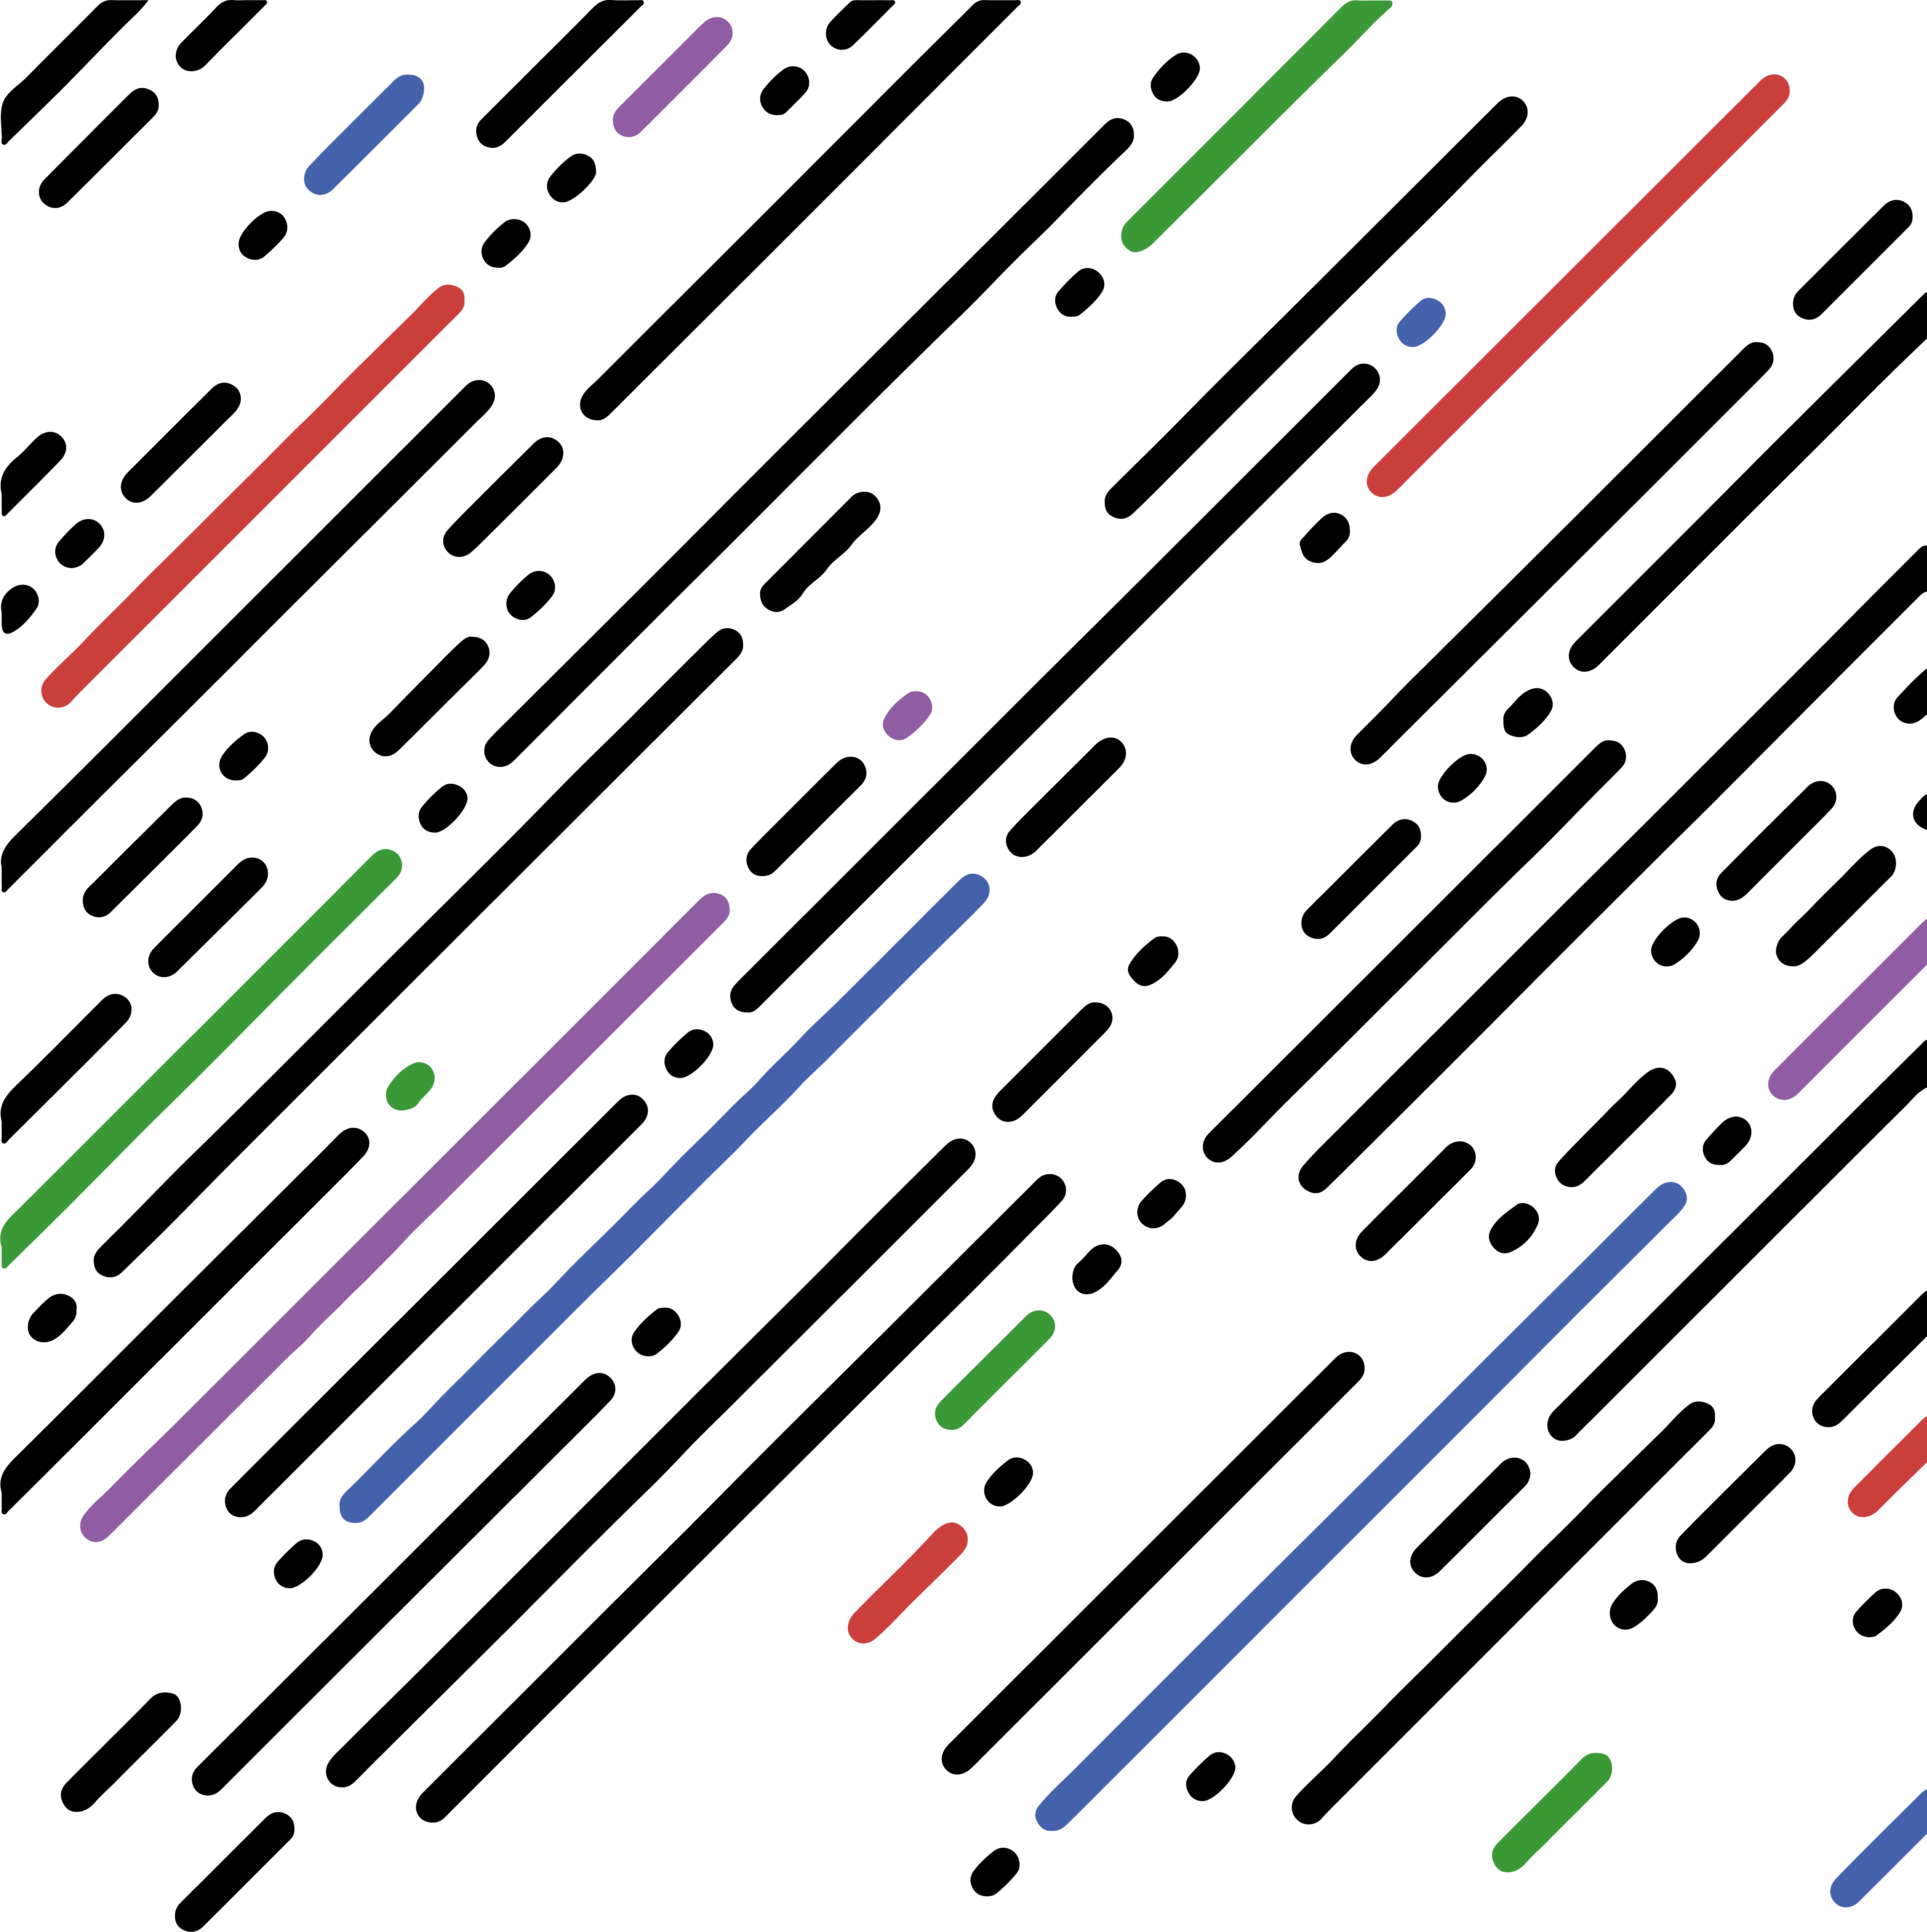
\includegraphics[width=\paperwidth]{capa.png}}; %Capa Imagem A4 21x29.7
\draw[anchor=north] (midpoint) node [fill=blue!50!white,fill opacity=0.0,text opacity=1,inner sep=1cm]{\Huge\centering\bfseries\sffamily\parbox[c][][t]
        {\paperwidth}
        {\centering Introdu\c{c}\~{a}o \`{a} Linguagem Julia\\[5pt] % Titulo Livro
{\Large Paradigmas de Linguagens de Programa\c{c}\~{a}o}\\[20pt] % Subtitle
{\huge  \color{purple} Daniel Brito dos Santos}\\ % Autor nome
{\huge  \color{purple}  Ausberto S. Castro Vera}\\
{\small \today}
}}; % Autor nome
\end{tikzpicture}};

\end{tikzpicture}
\vfill
\endgroup

%----------------------------------------------------------------------------------------
%	COPYRIGHT PAGE
%----------------------------------------------------------------------------------------

\newpage
~\vfill
\thispagestyle{empty}

\noindent Copyright \copyright\  \the\year{} Daniel Brito dos Santos e Ausberto S. Castro Vera\\ % Copyright notice

\noindent \textsc{UENF - Universidade Estadual do Norte Fluminense Darcy Ribeiro}\\ % Universidade

\noindent \textsc{CCT - Centro de Ci\^{e}ncia e Tecnologia}\\ % Centro
\noindent \textsc{LCMAT - Laborat\'{o}rio de Matem\'{a}ticas}\\ % Laboratorio
\noindent \textsc{CC - Curso de Ci\^{e}ncia da Computa\c{c}\~{a}o}\\ % Curso

%\input{autor.tex} \\

\noindent \textit{Primeira edi\c{c}\~{a}o, Maio 2019} % Printing/edition date

%----------------------------------------------------------------------------------------
%	TABLE OF CONTENTS
%----------------------------------------------------------------------------------------

\chapterimage{sumario.png} % Table of contents heading image

\pagestyle{empty} % No headers

\addtocontents{toc}{\protect{\pdfbookmark[0]{\contentsname}{toc}}}
\tableofcontents % Print the table of contents itself

\cleardoublepage % Forces the first chapter to start on an odd page so it's on the right

\pagestyle{fancy} % Print headers again

%----------------------------------------------------------------------------------------
%	PART
%----------------------------------------------------------------------------------------
%\part{Part One}

%----------------------------------------------------------------------------------------
%	CHAPTERS
%----------------------------------------------------------------------------------------
\chapterimage{capitulo01.jpg} % Chapter heading image
% Prof. Dr. Ausberto S. Castro Vera
% UENF - CCT - LCMAT - Curso de Ci\^{e}ncia da Computa\c{c}\~{a}o
% Campos, RJ,  2021
% Disciplina: Paradigmas de Linguagens de Programa\c{c}\~{a}o
% 



\chapter{ Introdu\c{c}\~{a}o}


A linguagem Julia surgiu com o objetivo de solucionar o que seus criadores chamaram de "problema das duas linguagens" na computação científica \cite{Bezanson2012}. Ele se refere ao fato, detalhado por \cite{Balbaert2016}, de muitos cientistas, engenheiros e matemáticos usarem uma linguagem flexível e amigável como Python, R, ou Matlab, que os permite focar no problema sendo investigado ao invés de detalhes de implementação computacional. Pois tais linguagens têm uma estrutura interna que permite uma sintaxe com maior nível de abstração, tornando a escrita de programas mais simples e expressiva \cite{Fangohr2004}. Porém, essa estrutura facilitadora tem um custo de performance muitas vezes proibitivo em relação aos programas escritos em linguagens como C e Fortran \cite{Nanz2015}. 
Dessa forma, segundo \cite{Balbaert2016}, muitas vezes um fluxo de trabalho é desenvolvido em uma linguagem dinâmica com uma amostra dos dados para em seguida ser implementado em uma linguagem mais performática e só então exercer sua finalidade com a totalidade dos dados ou acessível ao usuário final, chamado ambiente de produção. 

\cite{Klok2021} também aborda esse "problema das duas linguagens", em seu caso chamando de 

Não obstante, segundo seus criadores, a linguagem que vislumbraram iria além de resolver o "problema das fuas linguagens" dilema entre "velocidade de execução" e "velocidade de desenvolvimento" que \cite{Klok2021} menciona. Em seu artigo de lançamento eles afirmaram: 

\begin{quote}
   Criamos Julia, em resumo, porque somos gananciosos. 
   Queremos uma linguagem open source com uma licença liberal. Queremos a velocidade de C com o dinamismo de Ruby. Uma linguagem homoiconica com macros verdadeiras como Lisp, mas com notação matemática obvia e familiar como Matlab. Queremos algo tão geral quanto Python, tão fácil para estatística quanto R, tão natural para processamento de strings quanto Perl, tão poderoso para algebra linear quanto Matlab e tão bom como cola de programas quanto shell. Algo estupidamente simples de aprender, e ainda assim deixe o mais sério dos hackers satisfeito. Queremos algo interativo e que seja compilado. 
   
   Mencionamos que deve ser tão rápida quanto C? 
   \href{https://julialang.org/blog/2012/02/why-we-created-julia/}{[Why We Created Julia, 2012]}  \cite{Bezanson2012a}
   
   
\end{quote}

Assim, de acordo com \cite{Bezanson2017}, em 2012 foi lançada Julia, uma linguagem compilada para código nativo eficiente, tipagem dinâmica, que permite expressar paradigmas procedural, funcional, orientação a objetos e metaprogramação.  Além de suporte nativo e de alto nível ao paralelismo, alta integração com as extensas bibliotecas já disponíveis para as linguagens que a inspiraram, suporte a um subconjunto do unicode para nome de variáveis e funções, permitindo letras gregas e subscritos. 
Com código aberto e livre para uso privado, comercial, modificação e distribuição.
Especialmente pensada na computação científica mas ainda assim de propósito geral e sim, praticamente tão rápida quanto C. \cite{Lobianco2019,Bezanson2017}

 Nesse trabalho apresentamos uma breve introdução a linguagem Julia, sua história, principais aplicações, sintaxe e ecossistema. 


% Entretanto devido as limitações de tempo foi necessário uma abordagem breve, e voltada a pessoas que já tenham certa familiaridade com programação, entretato podemos recomendar para os iniciantes o livro tal, no qual abordará pontos que não foram considerados aqui.



\newpage
\section{Aspectos históricos da linguagem Julia}

\begin{figure}[H]
   \begin{center}
       \caption{Criadores da linguagem Julia} \label{criadores}
       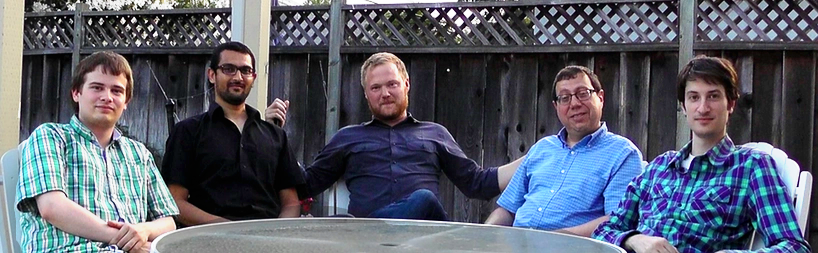
\includegraphics[width=12cm]{creators.png} \\
       {\tiny \sf Fonte: Julia Computing}
   \end{center}
  \end{figure}

Na Fig.\ref{criadores} vemos seus criadores da esquerda para a direita: Keno Fischer, Viral Shah, Stefan Karpinski, Alan Edelman, e Jeff Bezanson.
\newline

Assim como outras linguagens e construtos computacionais, muito de sua história tem pouco registro formal sendo a maior fonte seu site, blog e documentação oficiais, além de palestras em eventos técnicos e artigos jornalísticos, o que torna mais difícil uma reconstrução histórica precisa, não obstante, ressaltaremos os principais aspectos à seguir: 
%baseados em: (site julia) 
\begin{itemize}
   \item O nome Julia não tem nenhum significado, foi apenas um nome sugerido por um amigo de Benzanson que os criadores acharam bonito. \footnote{https://docs.julialang.org/en/v1/manual/faq/}
   \item O projeto da linguagem começou em 2009.
   \item Em \href{https://julialang.org/blog/2012/02/why-we-created-julia/}{2012} foi lançada para a comunidade open source. Segundo os criadores com 90\% das características que visionaram, inclusive inicialmente chamaram de Julia 1.0, mas posteriormente adiaram esse marco. 
   \item \href{https://julialang.org/blog/2014/08/julia-0.3-release/}{Julia 0.3} foi lançada em agosto de 2014 com melhorias na performance, e nas bibliotecas padrão, além de grande expansão no ecossistema de pacotes. 
   \item \href{https://julialang.org/blog/2015/10/julia-0.4-release/}{Julia 0.4} foi lançada em outubro de 2015 com refinamentos na linguagem e melhorias nas bibliotecas padrão, nesse momento haviam 700 pacotes registrados oficialmente.
   \item Nesse mesmo ano foi lançada a Julia Computing, Inc. considerando a necessidade de se ter uma companhia que oferecesse suporte, treinamento e consultoria na adoção da linguagem por big players. 
   \item \href{https://julialang.org/blog/2016/10/julia-0.5-release/}{Julia 0.5} no outubro de 2016, trouxe como principal novidade remover o custo de performace ao utilizar as funções anônimas, clausura, e funções de primeira ordem, conceitos fundamentais da programação funcional que a linguagem suporta desde o início. Trouxe também suporte arquiteturas ARM e Power, multi threading experimental, e simplificação no tipo string, dentre outras. 
   \item \href{https://julialang.org/blog/2017/06/julia-0.6-release/}{Julia 0.6} em junho 2017 com diversas pequenas mudanças tendo em vista aumentar a estabilidade e semântica da linguagem. 
   \item \href{https://julialang.org/blog/2018/08/one-point-zero/}{Julia 1.0}  dia oito de agosto de 2018, finalmente é lançada versão 1.0. Quase uma década de trabalho, mais de 700 pessoas contribuiram no código fonte, e milhares nos pacotes. Apresentou como principal característica a consolidação da linguagem, com essa base solidificada o foco passa a ser em construir sobre a fundação. Dentre as várias novidades podemos ressaltar o novo gerenciador de pacotes completamente refeito, representação canônica para missing values (valores faltantes) e tipo String seguro para dados arbitrarios, o que permite trabalhar com dados do mundo real sem o risco de depois de horas ou dias de processamento um caractere inválido levar a uma falha geral. 
   \item\href{https://julialang.org/blog/2020/08/julia-1.5-highlights/}{Julia 1.5} apresentou grande otimização na forma como seus Structs são alocados no heap, novas melhorias no multithreading, a possibilidade de selecionar o nível de otimização em cada módulo de modo a diminuir a famigerada latência da primeira execução. nova macro para chamar funções de C, gerador de números aleatórios 6 vezes mais rápido, e padronização do protocolo pkg. 
   \item\href{https://julialang.org/blog/2021/03/julia-1.6-highlights/}{Julia 1.6} em março de 2021 apresentou principalmente avanços na consolidação da linguagem, com diversas melhorias em diferentes aspectos que de modo geral trouxeram mais robustez e eficiência. 
\end{itemize}


\section{Áreas de aplicação da linguagem}
Júlia é atualmente utilizada por mais de 10 000 empresas, e 1 500 universidades, com 29 milhões de downloads e 87\% de  crescimento anual. \href{https://juliacomputing.com/}{(Julia Computing)}

Seus criadores ganharam os prestigiados prémios \href{https://news.mit.edu/2018/julia-language-co-creators-win-james-wilkinson-prize-numerical-software-1226}{MIT James H Wilkinson 2018} para Software Numérico e o \href{[https://www.computer.org/press-room/2019-news/2019-ieee-fernbach-award-edelman](https://www.computer.org/press-room/2019-news/2019-ieee-fernbach-award-edelman)}{IEEE Sidney Fernbach 2019} por "avanços extraordinários na computação de alta performance, algebra linear, computação científica e contribuições para a linguagem de programação Julia". 

Considerando ainda sua flexibilidade, simplicidade e performance, não é surpresa que tem crescido exponencialmente na computação científica, na computação de alta performance e também como linguagem de propósito geral \cite{Klok2021}. A figura \ref{clientes} mostra alguns dos principais clientes da linguagem.
\begin{figure}[H]
   \begin{center}
       \caption{Clientes da linguagem Julia} \label{clientes}
       
\includegraphics[width=12cm]{clientes.png} \\
       {\tiny \sf Fonte: Julia Computing}
   \end{center}
  \end{figure}


\subsection{Computação científica}

A computação científica consiste principalmente na análise e modelagem exploratória de determinado problema, o que necessita de um ferramental técnico específico e normalmente é feito por especialistas na área em questão. Nesse sentido, é fundamental que se tenha um ambiente adequado a prototipação, que suporte as demandas metodológicas e principalmente permita o máximo de expressividade do profissional de modo que ele não precise se especializar também em computação para desempenhar bem o seu trabalho. \cite{Kaw2000,Wilson2014,Perez2007}

Júlia foi feita sob medida com esse propósito, suprindo todas essas necessidades e ainda oferecendo uma notação matemática clara e intuitiva, com suporte nativo a construtos como matrizes, vetores, funções anônimas e de primeira ordem além das bibliotecas especializadas que implementam os métodos necessários de estatística, algebra linear, e equações diferenciais pra citar alguns exemplos. \cite{Klok2021}

Dessa forma temos visto um importante crescimento da linguagem nas áreas de Data Science, machine learning\footnote{https://juliacomputing.com/case-studies/princeton/}, 
economia \footnote{https://juliacomputing.com/case-studies/thomas-sargent/}, pesquisa operacional, e todas as ciências naturais como biologia, e física. \cite{Perkel2019,Udell2014}
%([]TODO citar cada biblioteca)

\subsection{Computação de alta performace}
Outra área na qual Julia se destaca é a computação de alta performace. Temos exemplos notáveis de uso nas mais diversas industrias como a financeira, farmacéutica\footnote{https://juliacomputing.com/case-studies/astra-zeneca/}, médica, aeroespacial \footnote{https://juliacomputing.com/case-studies/celeste/} dentre várias outras. 

Podemos destacar na industria financeira a análise de séries temporais no fundo de investimentos BlackRock\footnote{https://juliacomputing.com/case-studies/blackrock/}, o cálculo de risco junto ao banco britânico Aviva\footnote{https://juliacomputing.com/case-studies/aviva/}, modelos econômicos no Federal Reserve Bank of New York\footnote{https://juliacomputing.com/case-studies/ny-fed/}, e em nosso próprio BNDS no manejo de quase um trilhão de reais com modelos de otimização estocástica multi-estágios\footnote{https://juliacomputing.com/case-studies/bndb/}, em todas essas implementações ouve um aumento em pelo menos 10x na velocidade de processamento, em boa parte dos casos reduzindo quase a metade o número de linhas de código, o que aumenta exponencialmente a legibilidade, diminui os erros e aumenta a produtividade dos desenvolvedores. Na Aviva chegou a reduzir 93\% do código e aumentar em 1 000x a velocidade. 

Ela também foi utilizada no projeto Celeste onde atingiu a performance de 1.54 petaFLOPS, e entrou para o seleto panteão das linguagens que alcançaram essa magnitude: Fortran, C, C++ e Julia.\footnote{https://juliacomputing.com/media/2017/09/julia-joins-petaflop-club/}

Não atoa foi selecionada pela Aliança de modelagem climática como a única linguagem na sua próxima geração de modelos climáticos. Além de ser utilizada pela NASA e pelo INPE brasileiro no planejamento de missão e simulação de satélites. \footnote{https://juliacomputing.com/case-studies/BrazilNationalinstituteforspaceResearch/}



\subsection{Uso geral}

Apesar de ser particularmente utilizada em computação técnica, a linguagem Julia é de propósito geral, e também é utilizada em uma variedade de outras aplicações, como por exemplo para gerar sites estáticos por meio da biblioteca \href{http://franklinjl.org/)}{Franklin.jl}, interfaces cliente/servidor HTTP com \href{https://github.com/JuliaWeb/HTTP.jl}{HTTP.jl}, desenvolver aplicações gráficas com \href{https://github.com/JuliaGraphics/Gtk.jl}{Gtk.jl} ou binários multiplataforma para diversas arquiteturas com a \href{http://binarybuilder.org/}{BinaryBuilder.jl}

Também é interessante notar seu salto da 43ª para a 26ª posição no \href{https://www.tiobe.com/tiobe-index/}{TIOBE index}. 
Desse modo ela tem mostrado um crescimento orgânico e saldável, mesmo com uma proposta tão ambiciosa e sendo ainda tão jovem. Assim, podemos esperar muitas novidades paro o futuro, pois seu time original, agora expandido tanto em pessoas quanto em capital, tem recebido cada vez mais atenção na comunidade open souece. Além dos incentivos das mais importantes entidades de programação numérica e da industria. \footnote{https://www.fortuneita.com/2021/07/19/julia-computing-raises-24m-in-series-a-former-snowflake-ceo-bob-muglia-joins-board/} \footnote{https://www.hpcwire.com/off-the-wire/julia-computing-receives-darpa-award-to-accelerate-electronics-simulation-by-1000x/}




%\newpage

\chapterimage{capitulo01.jpg} % Chapter heading image
% Prof. Dr. Ausberto S. Castro Vera
% UENF - CCT - LCMAT - Curso de Ci\^{e}ncia da Computa\c{c}\~{a}o
% Campos, RJ,  2021
% Disciplina: Paradigmas de Linguagens de Programa\c{c}\~{a}o
%


\chapter{ Conceitos básicos da Linguagem Julia}

%Neste capítulo, buscamos apresentar de forma condensada e reestruturada o conteúdo de preparação de ambiente e tipos de dados presentes nos quatro principais livros da bibliogradia desse trabalho. 

Neste capítulo apresentamos os conceitos basais de sintaxe, design e ferramental necessários para se programar em Julia. Nesse sentido, todo o conteúdo dete capítulo foi baseado nos quatro principais livros-texto da bibliografia desse trabalho. Sendo eles, principalmente \cite{Lobianco2019} e \cite{Balbaert2016}, seguidos de \cite{Lauwens2019} e \cite{Kwong2020}.

\section{Preparação do ambiente}
%Faltando algo para conectar esse parágrafo ao anterior []
Para executar código Júlia, basta baixar e descompactar os arquivos binários no site oficial da linguagem. O arquivo executável apresenta o console de interpretação mostrado na figura \ref{REPL} (também conhecido como "REPL - Read, Eval, Print, Loop") por onde é possível executar Julia tanto por linha de comando quanto por meio de scripts .jl. Também é possível utilizar diversos ambientes de desenvolvimento integrado que serão abordados alguns capítulos adiante.
%Deveria colocar esse parágrafo em uma nova section? tipo first things first? []
\begin{figure}[H]
\begin{center}
    \caption{REPL Julia} \label{REPL}
    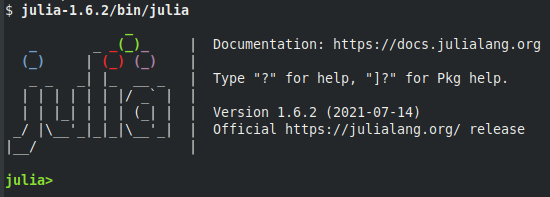
\includegraphics[width=12cm]{aplicacoes/ambiente.png} \\
    {\tiny \sf Fonte: Autor}
\end{center}
\end{figure} 

\subsection{Pacotes e módulos}

Os criadores da lingua escolheram construir um núcleo leve complementado por uma biblioteca padrão (Standard Library) distribuída junto dos binários, e um poderoso gerenciador de pacotes capaz de baixar (muitas vezes direto de repositórios GitHub), pré compilar, atualizar e resolver dependências de pacotes a partir de comandos simples. 

Para acessar o gerenciador de pacotes podemos importar o módulo de pacotes (import Pkg) e executar os comandos no formato Pkg.(ARGS). Demonstramos esse caso de uso na figura \ref{import_Pkg} onde executamos o comando para instalar o pacote Plots. Como o pacote já está instalado, o Pkg apenas o reconhece e não altera os pacotes.
%A figura \ref{import_Pkg} demonstra esse caso de uso ao tentarmos instalar o pacote Plots que como já está instalado, podemos observar que o Pkg reconhece tal fato e não altera nossos pacotes. 
Também podemos utilizar o modo especial de pacotes no REPL que traz algumas facilidades como autocompletar por exemplo. Nesse caso, basta digitar "]" para entrar nesse modo especial do REPL, como mostrado na figura \ref{pkg}. Na figura \ref{REPL_plots} repetimos o comando para instalar a biblioteca Plots, dessa vez no REPL. 
%Já no REPL também podemos apenas digitar ] para entrar no modo especial de pacotes, conforme a figura \ref{pkg}. nele temos algumas facilidades como autocomplete.
\begin{figure}[H]
\begin{center}
    \caption{Utilizando o Pkg em scripts} \label{import_Pkg}
    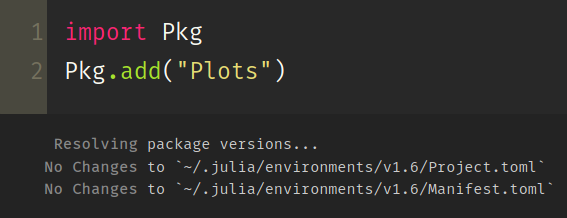
\includegraphics[width=12cm]{aplicacoes/import_Pkg.png} \\
    {\tiny \sf Fonte: Autor}
\end{center}
\end{figure} 

\begin{figure}[H]
\begin{center}
    \caption{REPL - modo pacotes} \label{pkg}
    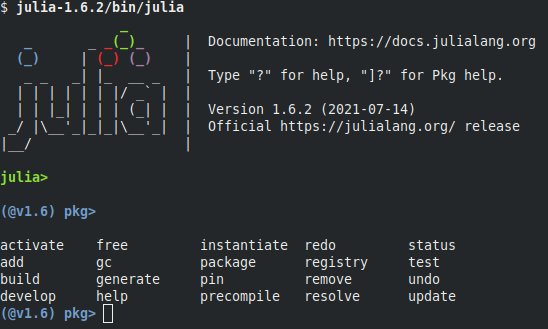
\includegraphics[width=12cm]{aplicacoes/pkg.png} \\
    {\tiny \sf Fonte: Autor}
\end{center}
\end{figure} 

\begin{figure}[H]
\begin{center}
    \caption{Utilizando modo Pkg do REPL } \label{REPL_plots}
    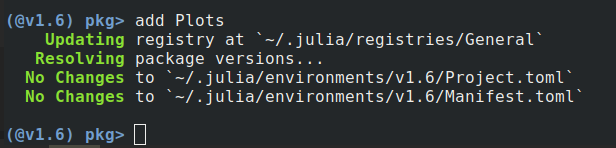
\includegraphics[width=12cm]{aplicacoes/REPL_plots.png} \\
    {\tiny \sf Fonte: Autor}
\end{center}
\end{figure}

Listamos a seguir alguns dos principais comandos do módulo Pkg. Em seguida demonstramos exemplos com o comando "status"  tanto no modo especial de pacotes do REPL (figura \ref{pacotes}) quanto em um exemplo de código Julia (figura \ref{Pkg_script}):
\begin{itemize}
  \item \textbf{status:} retorna uma lista (nome e versão) dos pacotes instalados localmente.
  \item \textbf{update:} atualiza o índice local de pacotes e os próprios pacotes para a versão mais recente.
  \item \textbf{add nomePacote:} automaticamente baixa e instala um pacote.
  \item \textbf{rm nomePacote:} remove o pacote e todas as suas dependências.
\end{itemize}

\begin{figure}[H]
\begin{center}
    \caption{Pkg.status no modo de pacotes do REPL} 
    \label{pacotes}
    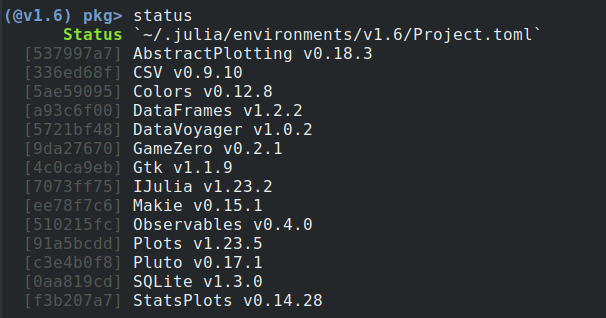
\includegraphics[width=12cm]{aplicacoes/pacotes.png} \\
    {\tiny \sf Fonte: Autor}
\end{center}
\end{figure} 
\begin{figure}[H]
\begin{center}
    \caption{Pkg.status em código Julia} 
    \label{Pkg_script}
    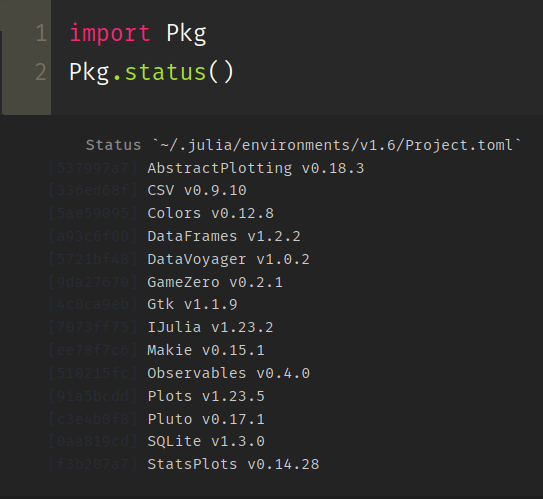
\includegraphics[width=12cm]{aplicacoes/Pkg_script.png} \\
    {\tiny \sf Fonte: Autor}
\end{center}
\end{figure} 

Uma vez instalado, para utilizar um pacote devemos utilizar um dos comandos seguintes:
\begin{itemize}
  \item \textbf{use:} permite acessar diretamente as funções de um pacote, basta adicionar o comando (using nomePacote) no inicio do script. 
  \item \textbf{import:} tem a mesma funcionalidade do use com a diferença de precisarmos nos referir ao nome completo da função (nomePacote.nomeFunção), o que tem a vantagem de manter a organização dos nomes. Via de regra, nesse caso definimos apelidos para os pacotes como por exemplo chamar o "Plots" de "pl" (const pl = Plots) %adicionar exemplo de código? []
\end{itemize}

%%Da mesma forma podemos usar (\textbf{use}) ou importar (\textbf{import}) qualquer arquivo Julia como módulo. Ele será analogamente executado ao ser invocado e qualquer símbolo definido estará disponível no escopo onde foi chamado. 

\subsection{Sistema de ajuda}
Além do sistema de pacotes, basta digitar "?"  para acessar o modo especial de ajuda do REPL. Assim, acordo com a documentação do termo buscado o sistema de ajuda pode retornar sua lista de métodos, exemplos de uso, descrição, lista de argumentos ou termos ou ainda os termos relacionados, conforme podemos ver na figura \ref{ajuda}. 
    \begin{figure}[H]
    \begin{center}
        \caption{REPL - modo ajuda} \label{ajuda}
        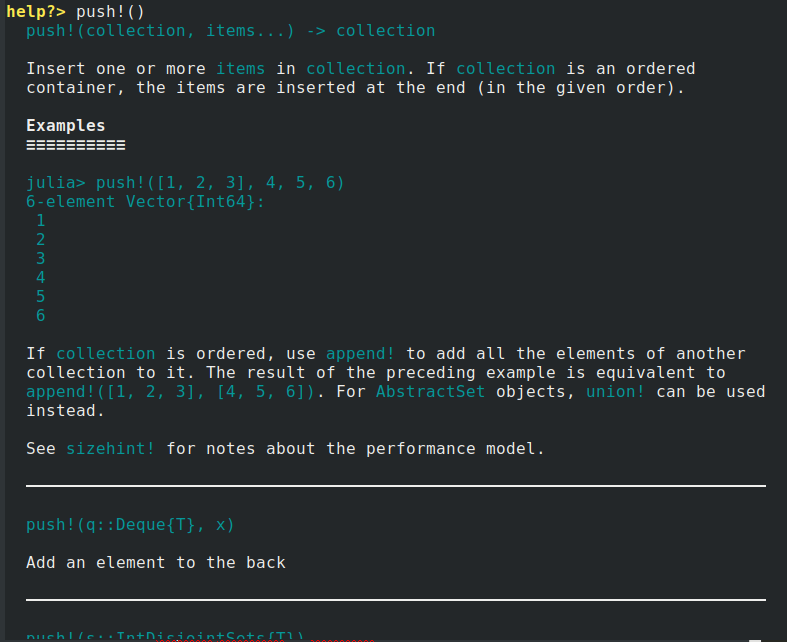
\includegraphics[width=12cm]{aplicacoes/help.png} \\
        {\tiny \sf Fonte: Autor}
    \end{center}
    \end{figure} 
%a linguagem também oferece um sistema de ajuda que retorna informação sobre o uso da maior partes das funções que pode ser acessado no REPL digitando "?" ou através do comando "?{termo de busca}". 

\subsection{Considerações gerais sobre sintaxe}
Ainda na preparação do ambiente para se programar, a sintaxe da linguagem é um ponto fundamental. Nesse sentido, listamos alguns desses aspectos gerais que consideramos importantes para se começar a programar em Julia: 

%é importante conhecer certos aspectos gerais da sintaxe da linguagem escolhida. A seguir, listamos as caracteristicas sintáticas gerais que julgamos serem mais relevantes para se começar a programar em Julia. 

%em Julia, alguns aspectos de sua sintaxe são importantes de se considerar. A seguir listamos os que achamos mais relevantes ao escopo do trabalho e futuos capítulos 

%Antes de abordamos as estruturas de dados e suas 
%A seguir listamos alguns pontos importantes da sintaxe de Julia. 
%Adicionar exemplos em código? []
\begin{itemize}
    \item Podemos adicionar ao código comentários de uma linha (\#) ou de múltiplas linhas (\#= =\#) que podem ser aninhados e colocados em qualquer lugar como mostra a figura \ref{comentarios}.

    \item Blocos não precisam de parênteses, utilizamos a palavra "end" para indicar o fim de um bloco, conforme figura \ref{blocos_identacao}.
    \item Espaços são sintaticamente significantes, identação, não. (Fig \ref{blocos_identacao}).
    \item Nomes de variáveis aceitam um subconjunto dos simbolos Unicode como letras gregas e até emojis. (Fig \ref{emoji})
    \item Vetores iniciam com o índice 1. (Fig \ref{indice})
    \item Por convenção, funções que podem alterar algum de seus argumentos têm um ponto de exclamação (!) no fim de seu nome. A função de ordenação (sort), por exemplo, recebe um vetor V desordenado e tem duas possibilidades: a função sort(V) retorna um vetor com os elementos de V ordenados, sem alterar o vetor V. Já a função sort!(V) ordena o próprio vetor, sem retorno. Podemos observar essa diferença na figura \ref{exclamacao}.
    \item O ponto e vírgula (;) é utilizado para suprimir o output de um comando ou acessar o shell (a partir do REPL) como apresentado na figura \ref{supressao}.
    
  \end{itemize}
    
    \begin{figure}[H]%comentarios
    \begin{center}
        \label{comentarios}
        \caption{Comentários em Julia} 
        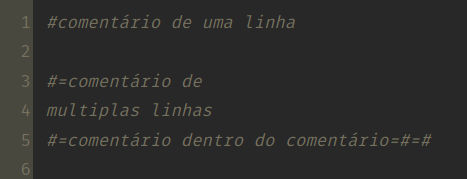
\includegraphics[width=12cm]{aplicacoes/comentarios.png} \\
        {\tiny \sf Fonte: Autor}
    \end{center}
    \end{figure} 

    \begin{figure}[H]%blocos
    \begin{center}
        \label{blocos_identacao}
        \caption{Blocos e identação em Julia} 
        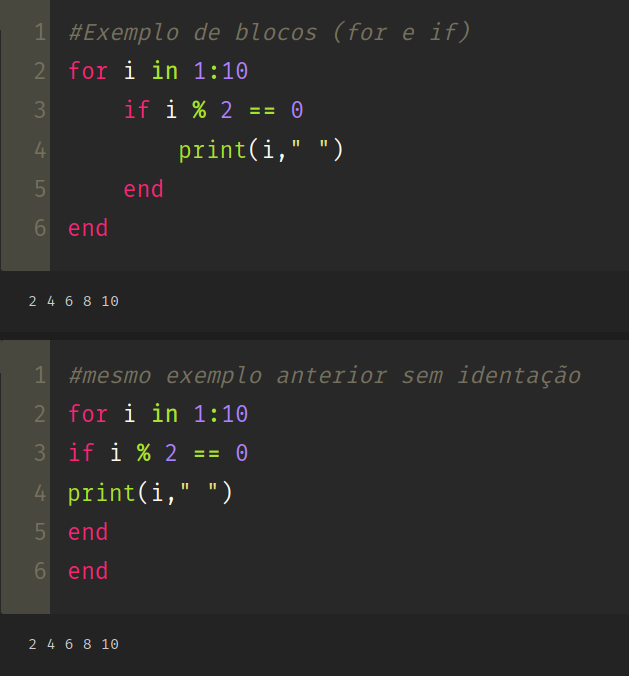
\includegraphics[width=12cm]{aplicacoes/bloco_identacao.png} \\
        {\tiny \sf Fonte: Autor}
    \end{center}
    \end{figure} 

%    \begin{figure}[H]%identacao
%    \begin{center}
%        \label{identacao}
%        \caption{Identação em Julia} 
%        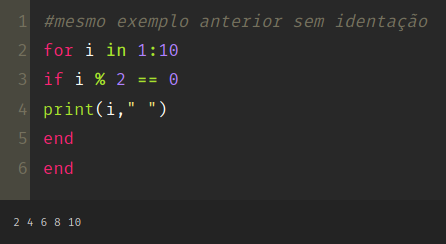
\includegraphics[width=12cm]{aplicacoes/identacao.png} \\
%        {\tiny \sf Fonte: Autor}
%    \end{center}
%    \end{figure} 
 
    \begin{figure}[H]%supressao
    \begin{center}
        \label{supressao}
        \caption{Supressão de output em REPL} %\label{REPL}
        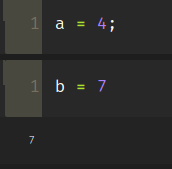
\includegraphics[width=6cm]{aplicacoes/supressao.png} \\
        {\tiny \sf Fonte: Autor}
    \end{center}
    \end{figure} 

    \begin{figure}[H]%emoji
      \begin{center}
        \label{emoji}
        \caption{Unicode nos nomes de variável} 
        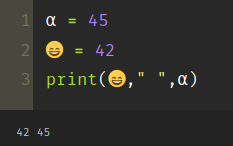
\includegraphics[width=6cm]{aplicacoes/emoji.png} \\
        {\tiny \sf Fonte: Autor}
    \end{center}
    \end{figure} 

    \begin{figure}[H]%indice
    \begin{center}
        \label{indice}
        \caption{Indices em Julia iniciam na posição 1} 
        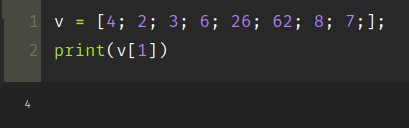
\includegraphics[width=12cm]{aplicacoes/indice.png} \\
        {\tiny \sf Fonte: Autor}
    \end{center}
    \end{figure} 

    \begin{figure}[H]%exclamacao
    \begin{center}
      \label{exclamacao}
      \caption{Diferença entre as funções sort() e sort!()} 
        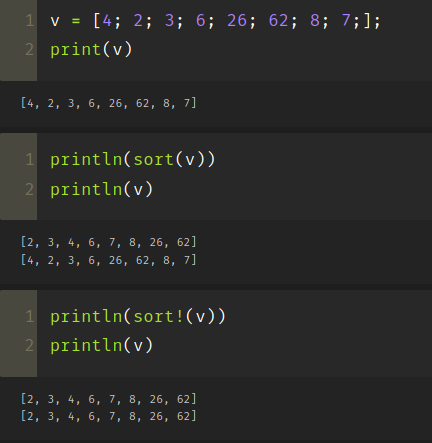
\includegraphics[width=12cm]{aplicacoes/exclamacao.png} \\
        {\tiny \sf Fonte: Autor}
    \end{center}
    \end{figure} 
\section{Tipos e estruturas de dados}
Segundo \cite{Lobianco2019}, Julia oferece nativamente um sistema hierárquico e bastante completo de tipos predefinidos que são divididos entre \textbf{escalares} e \textbf{coleções}.
Escalares são tipos atômicos, indivisíveis, como por exemplo inteiros, floats, e chars. Já as coleções são objetos que acomodam outros objetos como por exemplo vetores multidimensionais, dicionários e conjuntos. 
Nesta seção trazemos as ideias de \cite{Lobianco2019} e \cite{Balbaert2016} para organização e conteúdo dos diferentes tipos e estruturas de dados em Julia.

Nesse sentido, podemos destacar as seguintes características: 
\begin{itemize}
    \item Cada valor (mesmo os primitivos) tem seu tipo único, por convenção iniciando com letra maiúscula como Int64 e Bool (fig \ref{tipos_escalares}). 
    \item Na hierarquia dos tipos, o mais amplo é o tipo genérico Any.
    \item No caso de coleções e alguns escalares, o nome de seu tipo é seguido de chaves indicando os tipos dos elementos contidos, e sua dimensão, como por exemplo Array\{Int64,1\}, normalmente chamado de Vector\{Int64\}, ou seja uma coleção unidimensional de elementos do tipo Int64 como mostra a figura \ref{tipos_parametricos}. Na terminologia da linguagem são chamados tipos paramétricos.  
    \item Em Julia não existe divisão entre objetos e não-objetos pois todos os valores são objetos tipados, enquanto variáveis são apenas nomes relacionados a valores, portanto não têm tipo. 
   % \item Objetos do tipo coleção podem são denominados imutáveis quando não é possível alterar o seu valor (e valor de seus elementos), 
    \item Podemos converter objetos atraves da função "convert(T,x)", ou passar o objeto como argumento para uma função do tipo no formato "T(x)" como "Int64(x)" por exemplo, conforme a figura \ref{conversao} demonstra. 
    \item O operador :: pode ser utilizado para anexar anotações de tipo para expressões e variáveis conforme a figura \ref{anotacao_tipo}. \cite{Bezanson2017} afirma que essa anotação manual de tipos é totalmente opcional, pois apesar de haver situações nas quais ela se traduz em algum ganho de performance, na imensa maioria dos casos a inferência de tipos é suficiente para atingir eficiência máxima na compilação. Ainda assim a anotação de tipos é frequentemente utilizada para confirmar que um programa se comporta conforme o esperado. \label{anotacao_tipos}
    
\end{itemize}


    \begin{figure}[H]
    \begin{center}
        \caption{Tipos escalares de dados} \label{tipos_escalares}
        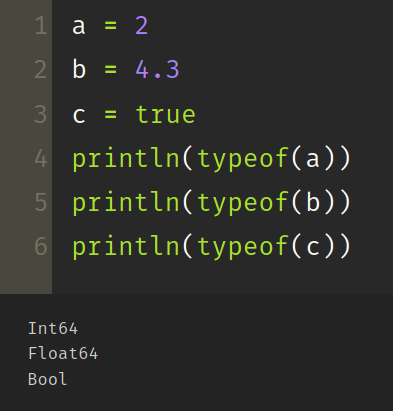
\includegraphics[width=10cm]{aplicacoes/tipos_simples.png} \\
        {\tiny \sf Fonte: Autor}
    \end{center}
    \end{figure} 

    \begin{figure}[H]
    \begin{center}
        \caption{Tipos paramétricos de dados} \label{tipos_parametricos}
        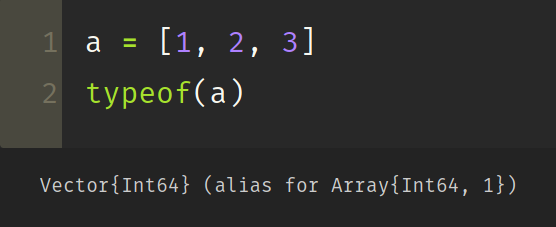
\includegraphics[width=12cm]{aplicacoes/tipos_parametricos.png} \\
        {\tiny \sf Fonte: Autor}
    \end{center}
    \end{figure}

    \begin{figure}[H]
    \begin{center}
        \caption{Conversão de tipos} \label{conversao}
        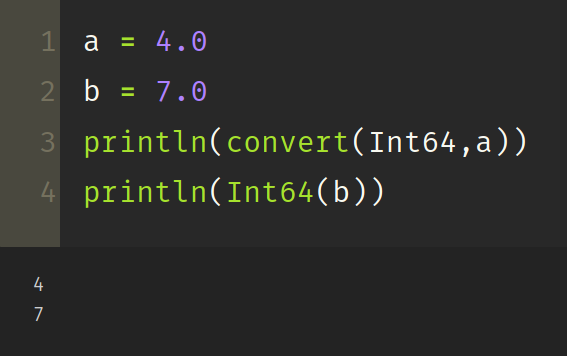
\includegraphics[width=12cm]{aplicacoes/convert.png} \\
        {\tiny \sf Fonte: Autor}
    \end{center}
    \end{figure}


    \begin{figure}[H]
    \begin{center}
        \caption{Anotação de tipos} \label{anotacao_tipo}
        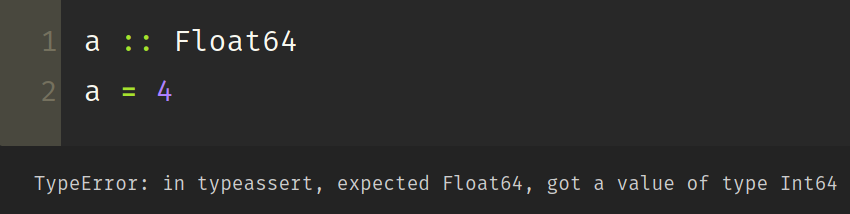
\includegraphics[width=12cm]{aplicacoes/type_annotation.png} \\
        {\tiny \sf Fonte: Autor}
    \end{center}
    \end{figure} 

    \subsection{Tipos simples}
    \begin{itemize}
      \item Caracteres individuais são do tipo Char, e representado por aspas simples.
      \item Booleanos são do tipo Bool, apenas com as instâncias True e False. Em um contexto de inteiros, booleanos podem ser interpretados como 0 e 1, assim como os inteiros 0 e 1 podem ser interpretados como booleanos, conforme é demonstrado na figura \ref{bool}.  
      %porém o oposto não ocorre (if 0 gera o erro de tipo "non-Boolean used in Boolean context"
    \item O tipo padrão de inteiro é o Int64 (existem outros 9 tipos inteiros) capaz de armazenar valores entre $-2^{63}$ e $2^{63-1}$.
    \item De modo análogo o padrão de ponto flutuante é o Float64.
    \item Números complexos são suportados pela variável global im que representa a raiz quadrada de -1 (fig \ref{complex}).
  \end{itemize}
 
    \begin{figure}[H]
    \begin{center}
        \caption{Tipo Bool} \label{bool}
        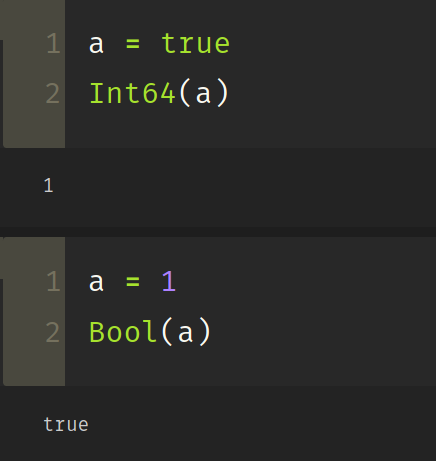
\includegraphics[width=8cm]{aplicacoes/bool.png} \\
        {\tiny \sf Fonte: Autor}
    \end{center}
    \end{figure} 

  \begin{figure}[H]
  \begin{center}
      \caption{Números complexos} \label{complex}
      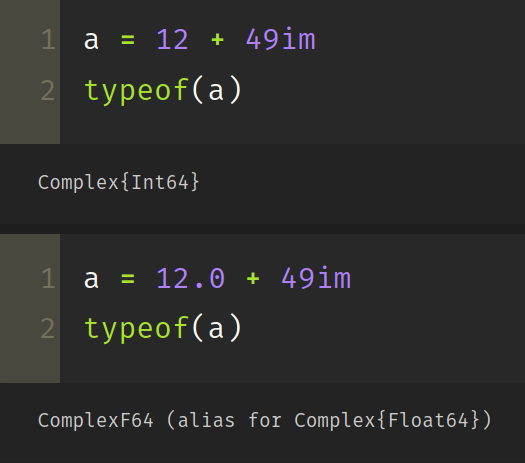
\includegraphics[width=12cm]{aplicacoes/complex.png} \\
      {\tiny \sf Fonte: Autor}
  \end{center}
  \end{figure} 

\subsection{Operações básicas}
Além dos operadores padrões de soma, subtração, multiplicação e divisão (+, -, *, /) temos a potenciação através do circunflexo ("3\^{}2"), a raiz quadrada por meio da função "sqrt()", o resto pelo operador \%, e a divisão inteira pelo símbolo $\div$ ("\textbackslash div" + tab), conforme apresentamos na figura \ref{operacoes}. 

    \begin{figure}[H]
    \begin{center}
        \caption{operacoes} \label{operacoes}
        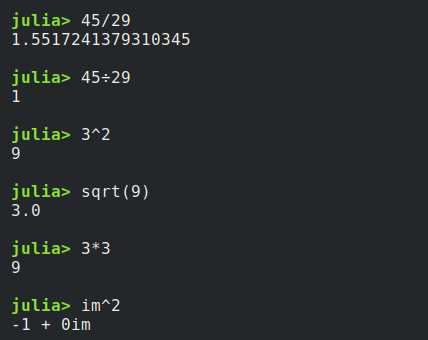
\includegraphics[width=12cm]{aplicacoes/operacoes_basicas.png} \\
        {\tiny \sf Fonte: Autor}
    \end{center}
    \end{figure} 



\subsection{Arrays}
Arrays (Array\{T, n\}) são coleções indexadas de objetos de tipo T, com n dimensões. %Isto é, um array acomoda elementos em ordem 
 Eles podem conter elementos de apenas um tipo (T), sendo que T pode ser de algum dos tipos que já abordamos (como inteiros e floats) ou dos tipos especiais \textbf{Any} ou \textbf{Union{}}.
 
 O tipo genérico Any tem a vantagem de permitir arrays genéricos Array\{Any,n\} com elementos de quaisquer tipos diferentes, entretanto, de acordo com \cite{Lobianco2019} são consideravelmente menos performáticos que arrays de tipos definidos. Isto porque para tipos definidos o compilador da linguagem é capaz de gerar código específico e otimizado para os tipos em questão, até mesmo para arrays do tipo Union\{$T_1,...,T_n$\}, que comportam elementos de cada um dos tipos $T_i$ definidos. O que não é possível para arrays do tipo Any.  
 %heterogêneos -nesse caso tendo o tipo genérico (Any) que em geral é consideravelmente menos performático- ou ser do tipo união (Union\{$T_1,T_2$\}) de outros tipos (exemplo: Union\{Int64,String\}), que consegue ter performace próxima do monotipo a partir dessa restrição.
 Alguns tipos de arrays recebem nomes especiais como por exemplo os vetores (Vector\{T\}) que são vetores unidimensionais, as matrizes (Matrix\{T\}) que são vetores bidimensionais e as Strings que são ainda um subtipo de vetor de caracteres. 

%Além das Strings que são vetores imutáveis de caractéres, também temos os tipos especiais Vector\{T\} e Matrix\{T\} que são respectivamente Arrays de uma e duas dimensões.

\subsubsection{Criação de Array}
Existem diversas formas de criarmos um Array do tipo T:
\begin{lstlisting}
     a  = [1;2;3] #cria um vetor coluna de uma dimensao.
     a = [1 2 3] #cria um vetor linha de uma dimensao.
     a = [] #cria um Array{Any,1}
     a = Int64[] #constroi um vetor de Int64 com uma dimensao.
     a = Array{Int64,1}() #mesmo do anterior, usando construtor.
     a = zeros(n) #cria um Array{Float64,1}
     a = zeros(Int64,n) #cria um array do tipo Int64 com n zeros.
     a = fill(j,n) #vetor com n elementos j
     a = rand(n) #vetor preenchido com n numeros aleatorios
\end{lstlisting}

\subsubsection{Acessar elementos}
Podemos acessar subvalores de um array utilizando chaves para selecionar um elemento (a[2]) ou uma fatia de intervalo fechado (a[de:passo:até]) da seguinte forma:
\begin{lstlisting}
   a = [1 2 3 4 5 6 7] 
   a[4] #retorna 4
   a[1:3] #retorna os elementos 1,2,3
   a[1:2:end] #retorna 1 3 5 7
   a[end:-1:1] #retorna 7 6 5 4 3 2 1
\end{lstlisting}

\subsubsection{Principais funções}
A seguir apresentamos as principais função para trabalharmos com Arrays, é interessante notar que normalmente as funções que podem modificar algum de seus argumentos contém uma exclamação.
\begin{lstlisting}
  push!(a,b) #adiciona o elemento b no fim de a.
  append!(a,b) #adiciona os elementos de b em a,
  #identico ao push! caso b seja escalar

  c = vcat(1,[2,3],[4,5]) #concatena arrays

  pop!(a) #remove o ultimo elemento do array,
  popfirst!(a) #remove o primeiro elemento do array.
  deletat!(a,pos) #remove o elemento da posicao pos

  pushfirst!(a,b) #b no inicio de a.

  length(a) #=ou=# if a in b end #retorna o comprimento do vetor

  sort!(a) #ordena o vetor a.
  sort(a) #retorna a ordenado sem modificar o vetor original
  reverse(a) #retorna elementos de a invertidos

  unique!(a) #remove duplicatas modificando a.
  unique(a) #retorna a sem duplicadas. 
  in(b,a) #checa a existencia de b em a.

  a... #=operador "splat" coverte os elementos em 
  parametros para uma funcao.=#

  maximum(a) #=ou=# max(a...) #retorna o maior valor.
  minimum(a) #=ou=# min(a...) #analogo ao anterior.
  sum(a) #retorna a soma dos elmentos de a.
  cumsum(a) #retorna um vetor com a soma cumulativa de a.

  empty!(a) #esvazia um vetor coluna.
  b = vec(a) #transforma vtores linha em vetores coluna.
  shuffle(a) #=ou=# shufle!(a) #=embaralha aleatoriamente 
  os elementos de a.=# 
  (requer o modulo Random).=#

  isempty(a) #checa se um array esta vazio.

  findall(x ->  x == value, a) #=retorna o indice de todas
  as ocorrencias de x.=#
  deleteat!(a, findall(x ->  x == value, a)) #=deleta todas as 
  ocorrencias de x de a.=#

  enumerate(a) #retorna um iterador de pares (indice, elemento).
  zip(a,b) #retorna um iterador de pares (a_element,b_element).
\end{lstlisting}

\subsubsection{Arrays aninhados e multidimensionias}
Arrays multidimensionais são os objetos do tipo Array\{T,N\} sendo o número de dimensões N maior que um, enquanto Arrays Aninhados apresentam uma dimensão sendo pelo menos um de seus elementos outro Array, como por exemplo um vetor de vetores Array\{Array\{T,1\},1\}.

A principal diferença entre ambos é que em matrizes o número de elemento em cada coluna deve ser igual e as regras da Álgebra Linear são aplicáveis. 


Os elementos de Arrays aninhados podem ser acessados por chaves duplas (a[2][3]), Já os elementos de multidimensionais podem ser acessados com os índices de cada dimensão separados por vírgula (a[lin,col]). Para vetores colunas tanto a[2] quanto a[1,2] retornam o segundo elemento. 

Podemos contruir Arrays multidimensionais de modo análogo aos vetores, alias estes são um caso específico daqueles:
\begin{lstlisting}
  a = [[1,2,3] [4,5,6]] #cria por colunas
  a = [1 4; 2 5; 3 6] #cria por linhas
  a = zeros(In64,n,m,g) #=cria uma matriz nxmxg 
  preenchida com zeros.=#
  a = [3x + 2y + z for x in 1:2, y in 2:3, z in 1:2] 
  #=tambem podemos usar list comprehension.=#
\end{lstlisting}

Também temos funções particularmente úteis para trabalharmos com Arrays multidimencionais:
\begin{lstlisting}
  size(a) #retorna uma tupla com os damanhos de cada dimencao
  ndimns(a) #retorna o numero de dimensoes.
  reshape(a,nElementDim1, nElementsDim2,...,nElementDimN) 
  #redimensiona o array.
  dropdimns(a, dimns=(dimRemov1, dimRemov2) 
  #remove as dimensoes especificadas
  transpose(a) #=ou=# a' #transpoe vetores ou matrizes.
  hvat(col1,col2) #concatena horizontalmente
  vcat(row1, row2) # concatena verticalmente. 
\end{lstlisting}
\subsection{Strings}
As strings (String) em Julia são vetores imutáveis de caracteres, isto é: conforme apresentamos na figura \ref{string_imutavel}, não é possível alterar nenhum dos elementos de uma String. 
Elas são definidas com aspas duplas e, assim como vetores, suportam indexação e looping.

\begin{figure}[H]
\begin{center}
    \caption{String imutável} \label{string_imutavel}
    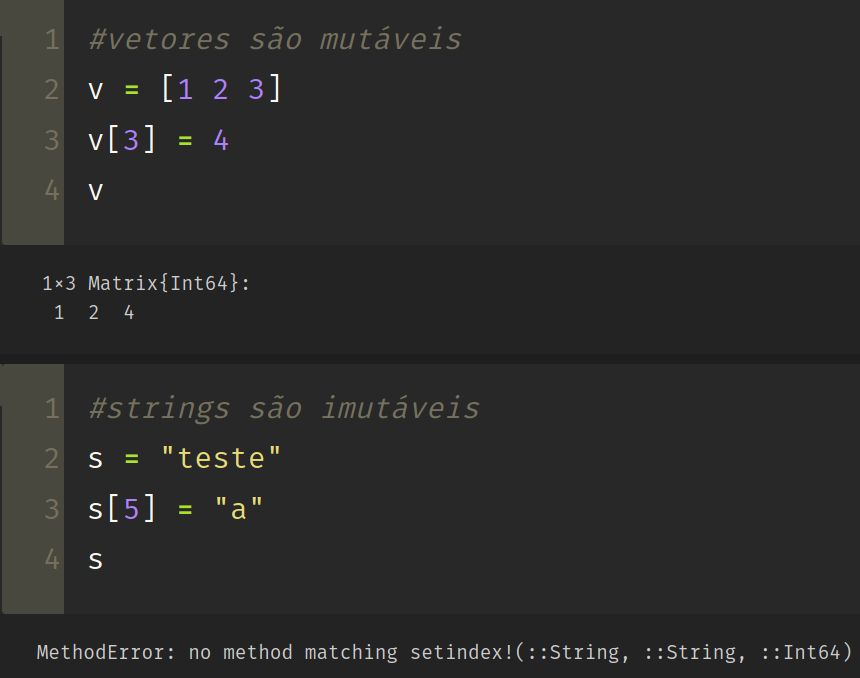
\includegraphics[width=12cm]{aplicacoes/string_imutavel.png} \\
    {\tiny \sf Fonte: Autor}
\end{center}
\end{figure} 

Algumas das operações típicas com strings são:
\begin{itemize}
    \item \textbf{split}(s, "\ ") nesse exemplo utiliza o espaço como um separador e retorna um vetor com as sublistas.
    \item \textbf{join}([s1,s2], "\ ") que une strings utilizando, nesse caso, o espaço entre cada junção.
    \item \textbf{replace}(s, {termo buscado} =  {substituto}) que substitui substrings compatíveis com a busca.
    \item \textbf{parse}(Int, "42") retorna a string convertida para um tipo numérico, no caso inteiro.
    \item \textbf{string}(123) retorna a string correspondente ao número.
    \item Existem três principais maneiras de concatenar strings:
        \subitem 
        \begin{lstlisting}    
  string("Hello, ","world")
  "Hello, World! The answer is $(43)"
  "Hello, " * "world"
        \end{lstlisting}
        
\end{itemize}


\subsection{Tuplas e Tuplas Nomeadas}
Tuplas (Tuple\{T1, T2,...\}) são grupos de tamanho fixo que contém valores separados por vírgula. Diferentemente de arrays, os valores de uma tupla não precisam ser do mesmo tipo, e esse fato não diminui sua performace visto que o tipo de uma tupla é uma tupla dos tipos de seus valores, análoga ao tipo Union{} como podemos observar na figura TAL. 
 Outra diferença em relação aos arrays é que tuplas são imutáveis, isto é, seus valores não podem ser modificados após a criação.   
 Podemos criar tuplas com parênteses ou sem conforme o exemplo:
\begin{lstlisting}
  t = (1, 2.5, "a")
  t = 1, 2.5, "a"
#Podemos converter uma tupla em um array:
  a = [t...] #utilizando o operador splat
  a = [i[1] for i in t] #utilizando list comprehension
  a = collect(t) #utilizando o operador collect. 
#De modo analogo podemos converter um array em uma tupla:
  t = (a...,)
\end{lstlisting}  
%\subsection{Tuplas nomeadas}
Já as Tuplas Nomeadas (NamedTuple) são coleções de itens que além do índice seus elementos, cada um deles pode ser identificado com uma chave única da seguinte forma: 
\begin{lstlisting}
  nt = (a=1,b=2.5) #define uma tupla nomeada
  nt.a #acessa o elemento a da tupla nt.
  keys(nt) #returna uma tupla com os nomes: (a,b)
  values(nt) #retorna uma tupla com os valores: (1, 2.5).
  collect(nt) #retorna um array com os valores.
  pairs(nt) #retorna um iterador dos pares (nome,valor) 
\end{lstlisting}

\subsection{Dicionários}
Dicionários (Dict\{Tkey, Tvalue\}) são coleções de valores relacionados a chaves únicas no formato (chave, valor). Apesar do mecanismo parecido com Tuplas Nomeadas, Dicionários são mutáveis e não retornam nem armazenam os pares chave-valor em ordem. 
%guardam mapas de chaves para valores com ordem aparentemente aleatória e diferente das Tuplas nomeadas, são mutáveis, tipo-instáveis.
Os principais métodos para trabalharmos com dicionários são:
\begin{lstlisting}
  d = Dict() 
  #cria um dicionario vazio.
  d = Dict{String,Int64}() 
  #cia um dicionario com tipagem definida para chaves e valores.
  d = Dict('a'= 1,'b'= 2, 'c'= 3) 
  #inicializa o dicionario com valores
  d[novaChave] = novoValor 
  #adiciona um novo par key-value ao dicionario.
  delete!(d,"chave") 
  #deleta o par correspondente a chave.
  map( (i,j) -  d[i]=j, ['a','b','c'],[1, 2 , 3]) 
  #adiciona pares de mapeamentos
  d["chave"] 
  #=retorna o valor correspondente a chave, 
  ou um erro caso ela nao exista.=#
  get(d, 'chave', "Chave inexistente") 
  #=retorna o valor da chave ou um valor padrao 
  caso ela nao exista.=# 
  keys(d) #retorna um iterator com todas as chaves de d.
  values(d) #retorna um iterador com todos os valores de d.
  haskey(d,"chave") 
  #retorna um booleano de acordo com a existencia da chave.
  in(('a'= 1), d) 
  #=checa se o par existe e a chave corresponde 
  ao valor especificado.=#

\end{lstlisting}

\subsection{Sets}
Usamos sets (Set\{t\}) para representar conjuntos mutáveis e sem ordem de valores únicos.
    \begin{lstlisting}
          s = Set() #=ou=# Set{T}() 
        #cria um set vazio
          s = Set([1,2,2,3,4]) 
        #inicializa com valores desconsiderando o 2 duplicado
          push!(s,5) 
        #adiciona elementos
          delete!(s,1)
        #deleta elementos
          intersect(s1,s2) 
        #intersessao de s1 e s2
          union(s1,s2) 
        #uniao de s1 e s2
          setdiff(s1,s2) 
        #diferenca entre s1 e s2
    \end{lstlisting}

\subsection{Números aleatórios}
Julia também facilita a obtenção de números pseudo aleatórios:
    \begin{lstlisting}
  rand()  
#retorna um float entre 0 e 1
  rand(a:b) 
#retorna um inteiro no intervalo [a,b]
  rand(a:0.01:b) 
#float aleatorio com precisao no segundo digito

#=Tambem podemos obter numeros de alguma distribuicao particular, 
desde que usemos o pacote Distributions=#

  rand(nomeDistribuicao[parametros])
  rand(Uniform(a,b))#por exemplo

#=Igualmente importante e a definicao da semente pseudo aleatoria
que permite termos um script reprodutivel:=#
  Random.seed!(1234) 
#define a semente pseudo-aleatoria para 1234
  Random.seed!() 
#reseta a definicao da semente

  rand(Uniform(a,b),2,3) 
#uma matriz 2x3 de numeros uniformemente aleatorios no 
intervalo [a,b].

    \end{lstlisting}
\subsection{Valores Faltantes}
Julia suporta, segundo \cite{Lobianco2019}, diversos conceitos de falta:
\begin{itemize}
    \item \textbf{nothing} (tipo Nothing) é o valor utilizado para blocos e funções que retornam nada. Conhecido como "null do engenheiro de software"
    \item \textbf{missing} (tipo Missing) representa um valor faltante no sentido estatístico, em que deveria haver um valor, apenas o desconhecemos. De modo que os containers e maioria das operações conseguem lidar eficientemente com esses casos. Também conhecido como "null do cientista de dados"
    \item \textbf{Nan} (tipo Float64) representa o resultado de uma operação que retorna é um "não-número". Similar ao missing no sentido de se propagar silentimente ao invés de gerar um erro. Analogamente Julia também oferece Inf (1/0) e -Inf (-1/0).
\end{itemize}
\section{Controle de fluxo e funções}
Em Julia nós temos as principais estruturas condicionais e repetitivas que encontramos nas linguagens mais populares. %devo citar diretamente os quatro livros novamente??
\subsection{Estrutura em bloco}
A sintaxe do controle de fluxo tipicamente se dá atráves de blocos que se iniciam com uma palavra chave seguida de uma condição (com parêntesis opcionais), e finalizam com a palavra "end" da seguinte forma: 
    \begin{lstlisting}
    <palavra chave>  <condicao> 
        #... conteudo do bloco....
    end 
    \end{lstlisting}
    \begin{lstlisting}
    #Por exemplo:
    for i in 1:5
        print(i)
    end     
    \end{lstlisting}
\subsection{Iteração repetida}
\subsubsection{For e while}
As funções for e while em Julia são muito flexíveis, suportando os contrutos padrões como percorer vetores, \textbf{break} que imediatamente aborta uma sequência e \textbf{continue} que imediatamente pula para a próxima iteração. Além de suportar condições múltiplas como demonstrado no exemplo abaixo. 
\begin{lstlisting}
for i=1:2, j=2:5
	println("i:$i, j:$j")
end
#=temos condicoes multiplas que geram um 
loop aninhado onde j percorre o intervalo 2:5 
para cada elemento i.=#

for i in "string exemplo"
	println(i)
end 
#=i percorrera cada caractere de "string exemplo" =#
\end{lstlisting}
\subsubsection{List comprehension}
List comprehension é essencialmente uma forma compacta de escrever um loop:
\begin{lstlisting}
a = [f(i) for i in [1 2 3]] 
#cria um array com f aplicada a cada elemento de [1 2 3]

[x+2y for x in [10,20,30], y in [1,2,3]]
#cria o array 
[d[i]=value for (i,value) in enumerate(lista)

[estudantes[nome] = idade for (nome,idade) in zip(nomes,idades)]
\end{lstlisting}
\subsubsection{Map}
Já a função Map aplica uma função a uma lista de argumentos.
\begin{lstlisting}
map((nome,idade) ->  estudantes[nome] = idade, nomes, idades)

a = map(f, [1,2,3]) 

a = map(x-> f(x), [1,2,3])
\end{lstlisting}

\subsection{Condicionais}
Condicionais em Julia também segue o design de similaridade com as linguagens que a inspiraram. Conforme demonstramos a seguir:
%Condicionais também são estruturados seguindo o design de simplicidade e similaridade com as linguagens dinâmicas:
\begin{lstlisting}
i = 5
if i == 1 
	println("i = 1")
elseif i == 2
	println("i = 2")
else 
	println("i nao e nem 1 nem 2")
end
\end{lstlisting}

As expressões são avaliadas até que seja possível inferir seu resultado (short circuited).%[] Pesquisar quão comun isso é
\subsubsection{Operador ternário}
Assim como list comprehension é uma forma concisa de escrever um loop, temos no operador ternário uma forma concisa de escrever um condicional:
\begin{lstlisting}
a? b: c
#se a eh verdadeiro execute b, do contrario execute c
\end{lstlisting}

\subsection{Funções}
Funções em Julia são muito flexíveis, podem ser delfinadas tanto em linha como em bloco quanto como funções lambda. Além disso, funções também são objetos, e portanto podem ser atribuídas a novas variáveis, retornadas como valores ou aninhadas:
\begin{lstlisting}
  f(x,y) = 2x+y
#definicao em uma linha
#-------------
  function f(x) 
  	2x + y 
  end
#definicao em bloco
#--------------
  x,y ->  2x + y
#funcao anonima
#--------------
  a = f
  a(5)
#funcao como objeto
\end{lstlisting}

As chamadas de funções em Julia seguem uma convenção conhecida como chamada por compartilhamento, que seria entre chamada por referência (onde um ponteiro a memória da variável é passado) e chamada por valor (onde uma cópia da variável é passada e a função trabalha nessa cópia).

Assim, as funções em Julia trabalham nas novas variáveis locais, conhecidas apenas dentro da função, de modo que atribuir a variável a outro objeto não vai influenciar o valor original, mas se o objeto ligado a variável é mutável a mutação do objeto também será aplicada a variável original:
\begin{lstlisting}
  function f(x,y) 
  	x = 10
  	y[1] = 10
  end
  x = 1
  y = [1,1]
  f(x,y)
#Resultado: x = 1, y = [10, 1]

\end{lstlisting}

Na comunidade Julia se recomenda seguir duas regras em relação a funções:%%[] ler no livro pra melhorar a coesão 
\begin{itemize}
    \item Que contenham todos os elementos necessários para sua lógica (sem acesso a nenhuma variável exceto seus parâmetros e constantes globais.)
    \item Que não alterem nenhuma outra parte do programa, ou seja, que não produza nenhum efeito colaterial além da eventual modificação de algum de seus argumentos. 
\end{itemize}

\subsubsection{Argumentos}
\begin{itemize} %%[] Adicionar exemplos em códigos
    \item Normalmente os argumentos são posicionais, mas temos o operador ponto e vírgula (;) para estabelecer que após o mesmo todos os argumentos sejam especificados por nome (keywords arguments)
    \item Os últimos argumentos podem ser especificados junto com valores padrão.
    %\item Também podemos declarar uma função de múltiplos argumentos.
    \item Funções podem receber um número variável de argumentos. 
    \item Também temos a opção de especificar os tipos dos argumentos.
    Como mencionado na sessão \ref{anotacao_tipos}, a principal razão para limitar os tipos dos parâmetros é para rapidamente evidenciar possíveis bugs. Pois assim, caso uma função seja acidentalmente chamada com um tipo diferente do planejado, ela retorna um erro de tipo ao invés de silentemente continuar a execução, que poderia ocasionar um erro de lógica mais difícil de detectar.
    %\item O retorno de uma função é opcional, podendo retornar um valor que pode ser normalmente retornam o último valor computado, mas podem retornar 
    \item Retornar um valor é opcional e normalmente as funções retornam o último valor computado, que pode inclusive ser de tipos coleção como uma tupla ou um array.
\end{itemize}
\begin{lstlisting}
  f(a,b=1;c=2) = (a+b+c) 
  f(1,c=3) 
#(1+1+3)

  function f(args...)
  	for arg in args
  		println(arg)
  	end
  end

  f(a::In64, b::Int64, c::Int64) = (a+b+c)

  f(a,b) = a*2,b+2
  x,y = f(1,2) 
# x = 2, y = 4
    
\end{lstlisting}

%\subsubsection{Multiple-Dispatch}
%Uma função pode ter múltiplos métodos para diferentes números e %tipos de inputs. Ao ser executada o computador selecionará a %implementação correta de acordo com os parâmetros na chamada da %função. Podemos listar todos os métodos de uma função com a função %methods(f).
%%Detalhar mais esse que é o coração da linguagem
% Prof. Dr. Ausberto S. Castro Vera
% UENF - CCT - LCMAT - Curso de Ci\^{e}ncia da Computa\c{c}\~{a}o
% Campos, RJ,  2021
% Disciplina: Paradigmas de Linguagens de Programa\c{c}\~{a}o
%


\chapter{Alma da linguagem}
A maior vantagem de Julia é a possibilidade de se ter código simultaneamente abstrato e eficiente. Essa característica definidora da linguagem emerge de aspectos fundamentais porém mais avançados de seu funcionamento, dos quais abordaremos os dois principais a seguir, baseado principalmente \cite{Balbaert2016} \cite{Kwong2020}.


%Neste capítulo abordaremos alguns dos aspectos avançados da %linguagem que são fundamentais à sua identidade, característica e %comportamento.
%
%[maybe] A maior vantagem de Julia é a possibilidade de se ter um %código simultaneamente abstrato e eficiente. Para compreender esse %DNA devemos observar três aspectos mais avançados da linguagem. 

\section{Compilação}
O segredo de sua velocidade reside na habilidade de gerar código especializado para diferentes tipos de inputs, aliada a capacidade ddo seu compilador inferir esses tipos. 

Isso porque Julia não tem um passo estático de compilação. O código de máquina é gerado em tempo de execução (JIT) por uma Máquina Virtual de de Baixo Nível (LLVM). Juntos esse sistema e o design da linguagem permitem que ela atinja máxima performance na computação cientifica, técnica e numérica. %(High Performace)

A chave dessa performance é a informação de tipo, que é feita por uma engine de inferência de tipos inteligente e totalmente automática que deduz os tipos baseada nos dados contidos nas variáveis (modelo *DataFlow*). Tanto que a declaração de tipos é opcional, msa pode ser feito para documentar o código, e dar pistas ao compilador para encontrar o caminho ótimo. %(High Performace)

Assim, na primeira vez executamos uma função Julia, ela é passeada para inferência de tipos, a seguir o JIT gera código LLVM que em seguida é otimizado e compilado para código de máquina. A partir da segunda execução, ela é executada diretamente em código de máquina. Podemos inspecionar ambos com as respectivas funções:%(High Performace)

\begin{lstlisting}
  code_llvm(f,(Int64))

  code_native(f,(Int64))
\end{lstlisting}

\section{Multimétodos}
A partir de sua poderosa inferência de tipos, Julia tem como paradigma principal o chamado Despacho Múltiplo (Multiple Dispatch) ou Multimétodos. Onde um sistema chamado *dynamic multiple dispatch* eficientemente seleciona o método ótimo para cada um dos argumentos de função dentre os vários métodos definidos. %(High Performace)

Assim, de acordo com o tipo é selecionada ou gerada uma implementação específica e extremamente eficiente em código nativo. %(High Performace)

Julia, portanto, leva a programação genérica e funções polimórficas ao limite, ao escrever o algoritmo uma vez e aplica-lo a uma amplo espectro de tipos, oferecendo funcionalidade comum a tipos drasticamente diferentes. Exemplo disso é a função genérica *size* que contem 50 implementações de métodos concretos. %(High Performace)

%\section{Metaprogramação}
% Prof. Dr. Ausberto S. Castro Vera
% UENF - CCT - LCMAT - Curso de Ci\^{e}ncia da Computa\c{c}\~{a}o
% Campos, RJ,  2021
% Disciplina: Paradigmas de Linguagens de Programa\c{c}\~{a}o
%


\chapter{Aplicações da linguagem}

Neste capítulo vamos apresentar cinco exemplos de aplicações escritas na linguagem Julia, bem como seus respectivos códigos-fonte, e imagens demonstrando seu funcionamento. 

\section{Quicksort}
A ordenação de elementos é uma das mais importantes operações computacionais. Assim, apresentamos uma implementação em Julia do Quicksort, um dos principais algoritmos de ordenação, que é inclusive o algoritmo utilizado na função nativa de ordenação da linguagem \href{https://github.com/JuliaLang/julia/blob/2364748377f2a79c0485fdd5155ec2116c9f0d37/base/sort.jl#L259-L296}{(sort())}.


%Desse modo apresentamos o Quicksort, dos principais algoritmos de ordenação, sendo, inclusive, utilizado por padrão na função de ordenação (\href{https://github.com/JuliaLang/julia/blob/2364748377f2a79c0485fdd5155ec2116c9f0d37/base/sort.jl#L259-L296}{sort!()}) nativa da linguagem. 
%\newline

Esse algoritmo se inicia elencando um elemento no vetor para ser o pivô dessa execução. 
A partir de então todos os elementos menores ou iguais ao pivô são colocados antes do mesmo e consequentemente todos os elementos maiores são colocados nas posições seguintes ao pivô. 

Em seguida é feito uma chamada recursiva da mesma função para cada uma dessas duas porções -do primeiro elemento até o anterior ao pivô, e do elemento seguinte ao pivô até o último. 

No Código \ref{quicksort_code}, apresentamos uma implementação do algoritmo disponível na wiki \href{https://rosettacode.org/wiki/Sorting_algorithms/Quicksort#Julia}{Rosetta Code}. 
Nela, o mecanismo principal de pivotagem se por meio de duas variáveis que guardam o último elemento da porção inferior ao pivo (left) e o primeiro elemento da porção superior ao pivô (right). Ou seja, os limites internos, visto que os limites externos serão os próprios primeiro e último elementos do vetor. 

Desse modo, essas variáveis dos limites internos se iniciam iguais aos limites externos, se aproximando do pivô da seguinte forma: 
caso o atual índice left seja menor que o pivo, o índice se desloca mais um elemento a direita.
Caso o atual índice right seja maior que o pivô ele se desloca para a esquerda.
Ambas ocorrem até que cheguem em um elemento fora de lugar, nesse caso o elemento fora de lugar em cada porção são permutados. 
Assim, temos duas porções para abrigarem os elementos maiores e menores que o pivô, que se iniciam vazias, mas vão avançando em direção ao pivô até que englobem todos os elementos. 

Na Fig.\ref{quicksort} implementamos o código no ambiente integrado de desenvolvimento (IDE) \href{https://code.visualstudio.com/docs}{Visual Studio Code} e demonstramos seu funcionamento com um vetor exemplo. 

[TODO: modificar o termo "listing" para algum outro?] 
\begin{lstlisting}[label={quicksort_code},caption={Implementação do algoritmo quicksort em Julia}]
  function quicksort!(A,i=1,j=length(A))
  if j > i
      pivot = A[rand(i:j)] 
      left, right = i, j
      while left <= right
          while A[left] < pivot
              left += 1
          end
          while A[right] > pivot
              right -= 1
          end
          if left <= right
              A[left], A[right] = A[right], A[left]
              left += 1
              right -= 1
          end
      end
      quicksort!(A,i,right)
      quicksort!(A,left,j)
  end
  return A
end
\end{lstlisting}

\begin{figure}[H]
   \begin{center}
       \caption{Quicksort na IDE VScode} \label{quicksort}
       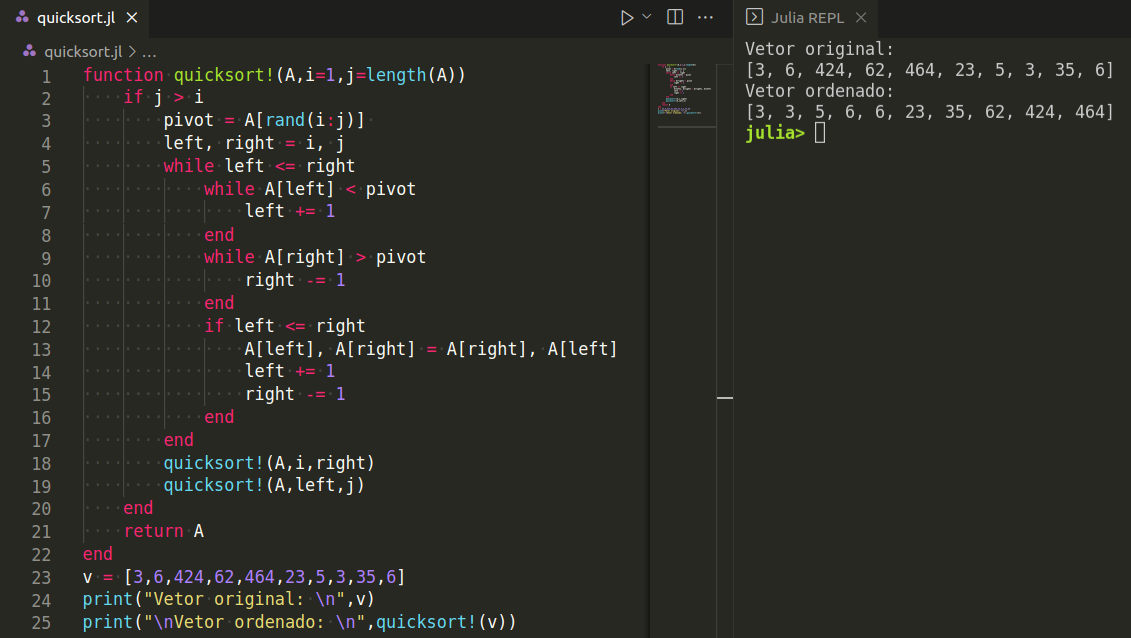
\includegraphics[width=12cm]{aplicacoes/quicksort.png} \\
       {\tiny \sf Fonte: Autor}
   \end{center}
\end{figure}

\section{Calculadora}
Outro aspecto muito importante da computação envolve o uso de interfaces gráficas para facilitar a interação do usuário com a máquina.
%, tanto no quesito acessibilidade quanto na acessibilidade de . 
Entretanto a construção de janelas, botões e afins é uma tarefa complexa, de modo que na maior parte dos casos os programadores utilizam uma biblioteca que implementa tais componentes de interface gráfica, sendo as duas mais famosas a Qt e a GTK chamadas de GUI Toolkit. %TODO refatorar esse parágrafo

Nesse exemplo demonstramos uma calculadora simples utilizando a biblioteca Gtk.jl que traz a biblioteca GTK de forma amigável para a linguagem Julia. 

O código \ref{calculadora_code} apresenta de modo compacto a implementação criada por Nand Vincchi que está disponível como exemplo no repositório \href{https://github.com/JuliaGraphics/Gtk.jl/blob/master/example/calculator.jl}{Github} da biblioteca Gtk.jl. 

Adicionamos as linhas para instalar o pacote Gtk, caso o mesmo ainda não esteja presente. O código original segue importando o pacote, e criando uma janela com título "Calculator", cria-se todos os botões, seguido de 4 chamadas "caixas" horizontais que são preenchidas com os botões criados. Cria-se uma caixa vertical para receber as quatro horizontais, a "tela" da calculadora, e espaços. Por sua vez essa caixa vertical é adicionada à janela.

Finalmente temos a função \_button\_clicked\_callback que adiciona responsividade dos botões de compor uma string que é apresentada na tela conforme são apertados, e ao clicar no igual a string construída é enviada a função "calculate" que a processa e retorna o resultado que será apresentado na tela.

Na figura \ref{calculadora} podemos ver a janela gráfica e parte do código sendo executado na IDE. 

\begin{lstlisting}[label={calculadora_code},caption={Calculadora simples em GTK}]
# Simple calculator application that utilises Gtk.jl
# created by Nand Vinchhi for GCI 2019

using Gtk

win = GtkWindow("Calculator")

b1 = GtkButton("1")
b2 = GtkButton("2")
b3 = GtkButton("3")
b_plus = GtkButton("+")
[...]
 
hbox1 = GtkButtonBox(:h)
hbox2 = GtkButtonBox(:h)
hbox3 = GtkButtonBox(:h)
hbox4 = GtkButtonBox(:h)

push!(hbox1, b1)
push!(hbox1, b2)
push!(hbox1, b3)
push!(hbox1, b_plus)
[...]

vbox = GtkBox(:v)
label = GtkLabel("")
GAccessor.text(label,"")

push!(vbox, GtkLabel(""))
push!(vbox, label)
push!(vbox, GtkLabel(""))
push!(vbox, hbox1)
push!(vbox, hbox2)
push!(vbox, hbox3)
push!(vbox, hbox4)
push!(win, vbox)

text = ""

function calculate(s)
	x = "+ " * s
	k = split(x)
	final = 0
	
	for i = 1:length(k)
		
		if k[i] == "+"
			final += parse(Float64, k[i + 1])
		elseif k[i] == "-"
			final -= parse(Float64, k[i + 1])
		elseif k[i] == "x"
			final *= parse(Float64, k[i + 1])
		elseif k[i] == "/"
			final /= parse(Float64, k[i + 1])
		end
	end
	return string(final)
end

function button_clicked_callback(widget)
	if widget == b1
		global text = text * "1"
        GAccessor.text(label, text)
    elseif widget == b2
    	global text = text * "2"
        GAccessor.text(label, text)
    elseif widget == b3
    [...]
        elseif widget == b_equalto
    	global text = calculate(text)
        GAccessor.text(label, text)
    end
end

id1 = signal_connect(button_clicked_callback, b1, "clicked")
id2 = signal_connect(button_clicked_callback, b2, "clicked")
id3 = signal_connect(button_clicked_callback, b3, "clicked")
[...]

showall(win)

\end{lstlisting}


\begin{figure}[H]
   \begin{center}
       \caption{Janela GTK da calculadora e vscode} \label{calculadora}
       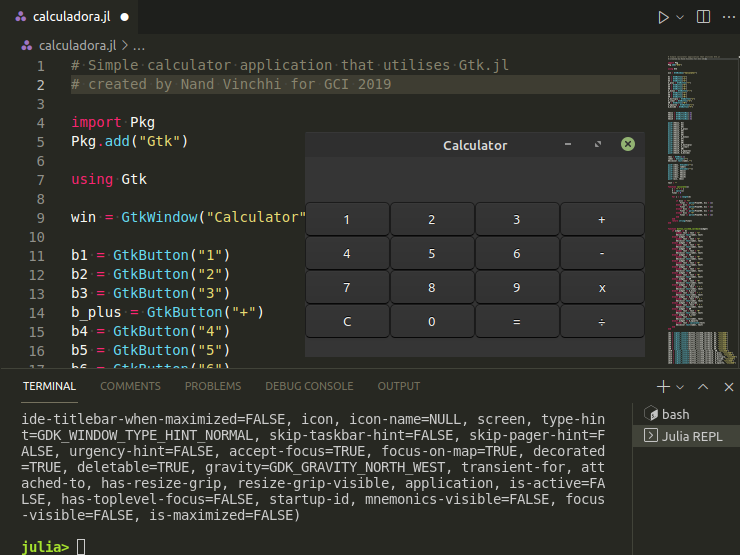
\includegraphics[width=12cm]{aplicacoes/calculadora.png} \\
       {\tiny \sf Fonte: Autor}
   \end{center}
  \end{figure}






\section{Plotagem (Iris data set)}
Igualmente importante no ecossistema Julia é a habilidade de analisar dados. Nesse exemplo demonstramos as funções básicas para ler um arquivo csv, utilizar um DataFrame, e plotar um gráfico que permita analisar esse dados. 

Para tanto, utilizamos o famoso Iris-dataset \cite{Fisher1936}, onipresente na literatura estatística e muito utilizado justamente para demonstrar um ecossistema de análise de dados. 

Esse dataset consiste na observação de 50 exemplares de três espécies de flores do gênero Iris (Fig. \ref{iris_flowers}), para cada observação temos o comprimento e largura de suas sépalas e pétalas bem como a qual espécie tais medidas pertencem (Fig.\ref{iris_data}).

\begin{figure}[H]
   \begin{center}
       \caption{Flores do gênero iris} \label{iris_flowers}
       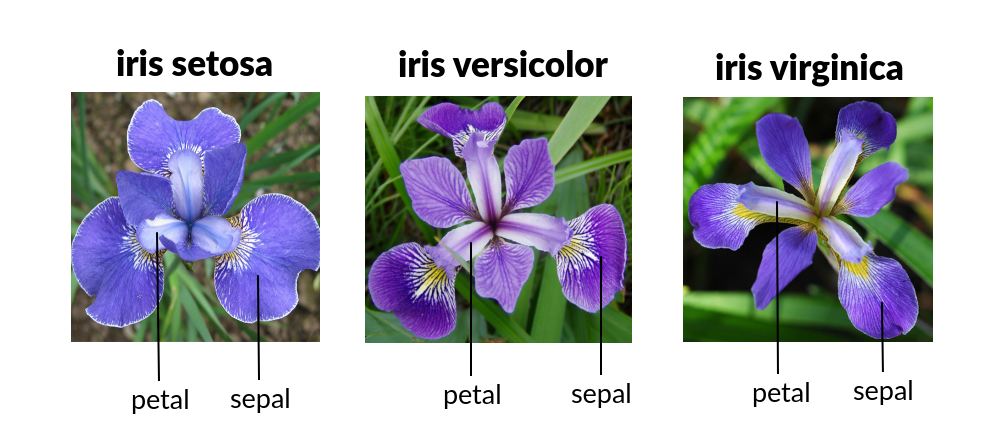
\includegraphics[width=12cm]{aplicacoes/iris-flowers.png} \\
       {\tiny \sf Fonte: https://rpubs.com/mbatista/545937}
   \end{center}
\end{figure}

\begin{figure}[H]
   \begin{center}
       \caption{Iris Dataset} \label{iris_data}
       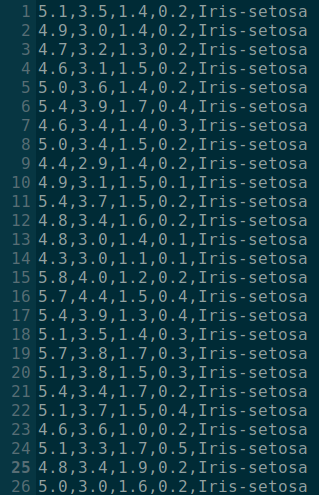
\includegraphics[width=5cm]{aplicacoes/iris_data.png} \\
       {\tiny \sf Fonte: https://archive.ics.uci.edu/ml/datasets/Iris/https://archive-beta.ics.uci.edu/ml/datasets/iris}
   \end{center}
\end{figure}

Assim, utilizamos o ambiente de desenvolvimento \href{https://jupyter.org/}{Jupyter Notebook}, que consiste em cadernos compostos por células interativas. 
Na figura \ref{iris_pacotes} temos a instalação dos pacotes: CSV para a leitura do arquivo com os dados, DataFrame que é a estrutura de dados padrão em tabelas, e DataVoyager que apresenta uma interface simples e interativa para plotagem exploratória de gráficos.

\begin{figure}[H]
   \begin{center}
       \caption{Instalação das bibliotecas} \label{iris_pacotes}
       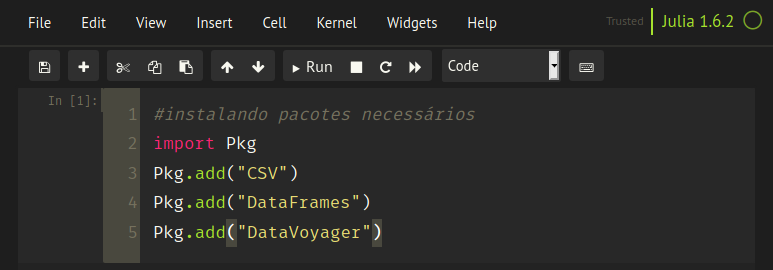
\includegraphics[width=12cm]{aplicacoes/iris_pacotes.png} \\
       {\tiny \sf Fonte: Autor}
   \end{center}
\end{figure}

Na figura \ref{iris_csv} importamos as bibliotecas CSV e DataFrames, criamos uma variável com o cabeçalho das colunas e finalmente lemos o arquivo csv e o armazenamos em memória na variável "iris". No retorno podemos ver parte do dataframe.

\begin{figure}[H]
   \begin{center}
       \caption{Leitura do CSV} \label{iris_csv}
       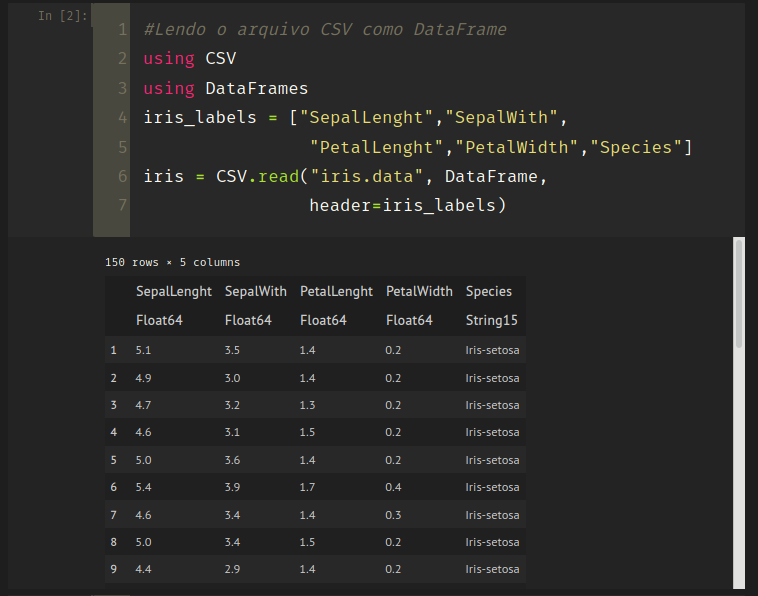
\includegraphics[width=12cm]{aplicacoes/iris_CSV.png} \\
       {\tiny \sf Fonte: Autor}
   \end{center}
\end{figure}

Já na figura \ref{iris_plot} temos a interface do DataVoyager, onde selecionamos o comprimento e largura das pétalas para os eixos bem como que a cor de cada ponto se dá de acordo com a espécie relacionada aquele ponto. O programa automaticamente nos retorna um scatter plot, conforme nossas especificações, e ainda sugere outras abordagens. 


\begin{figure}[H]
   \begin{center}
       \caption{Plotagem com DataVoyager} \label{iris_plot}
       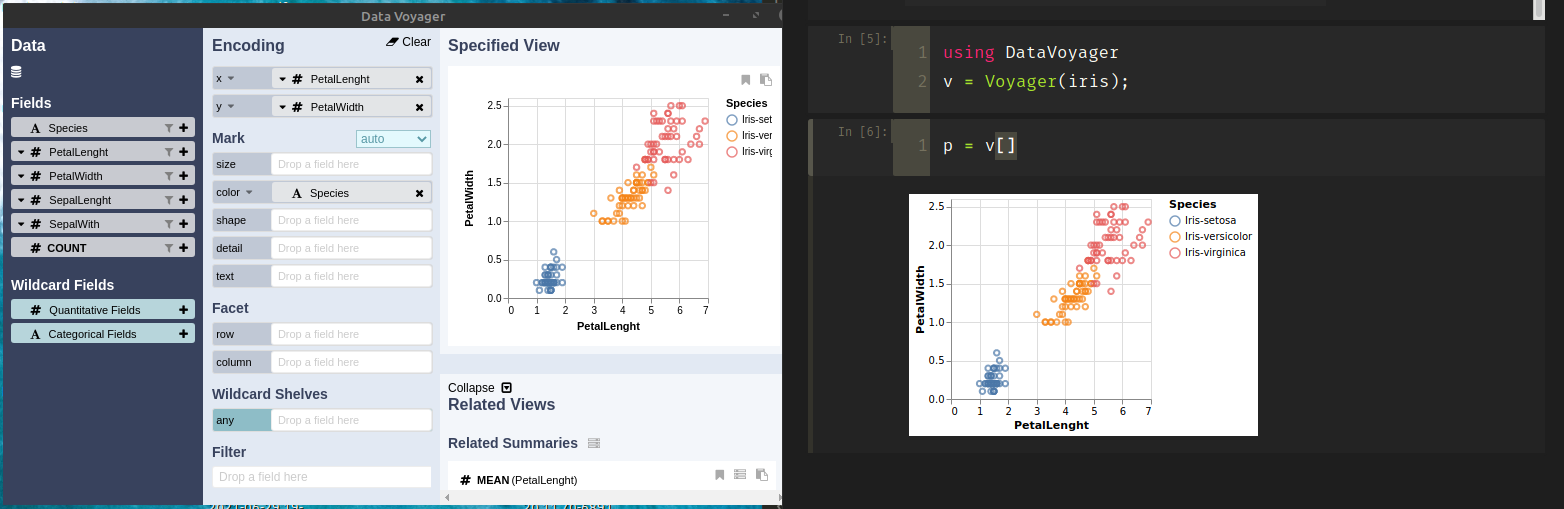
\includegraphics[width=15cm]{aplicacoes/iris_plot.png} \\
       {\tiny \sf Fonte: Autor}
   \end{center}
\end{figure}

Assim, torna-se evidente o potencial da linguagem e suas ferramentas para a análise exploratória de dados e construção de visualizações. 

%\subsection{texto removido da seção principal}
%em dados esse é o equivalente ao "hello, world!", o conjunto de dados das dimensões espaciais de três especies de flores coletada por ninguém menos que R.A Fisher, um dos pais da estatística. A ideia é que a facilidade de se trabalhar com esse conjunto de dados nos permite conhecer o ecossistema de dados de uma linguagem. 

%Desse modo, intalamos os pacotes necessários (Fig TAL), isto é, CSV para ler o arquivo, DataFrames para utilizarmos essa estrutura de dados, e o DataVoyager para explorar os dados e construir interativamente uma plotagem que nós permita compreender a relação entre as métricas e suas respectivas espécies. 

%Para tanto, baixamos o \href{https://archive.ics.uci.edu/ml/datasets/Iris/https://archive-beta.ics.uci.edu/ml/datasets/iris}{dataset}, utilizamos a biblioteca CSV para ler o arquivo e salva-lo como DataFrame na memória, em seguida utilizamos a biblioteca Plots para graficar os dados das flores.
% de modo a permitir futuras abordagens na busca matematicamente classificar uma dessas flores partindo apenas das dimensões de suas pétalas e sépalas. 
%"hello, world!" da programação, 
%Igualmente importante é a capacidade plotar gráficos, nesse exemplo nos usamos a função nativa de ler arquivos CSV 

%É possível classificar uma dessas flores tão parecidas apenas a partir das dimensões de altura e largura de suas sepas e petálas. 

\section{Banco de Dados SQL lite}
Outro aspecto fundamental de uma linguagem é a sua integração com banco de dados. Aqui trazemos um exemplo simples da criação e uso de um banco de dados SQLite, por meio da sua biblioteca disponível em Julia. 

Após instalarmos o pacote SQLite.jl, criamos um objeto e arquivo de banco de dados. Em seguida construímos uma função que lê o input padrão do teclado, separa a frase do autor e armazena ambos no banco de dados criado, conforme demostra e explica a figura \ref{sql_corpo}.
Esse código foi inspirado no seguinte exemplo disponível no Github. \footnote{https://github.com/julia4ta/tutorials/blob/master/Series\%2004/Tutorial\%2004x05/sourcecode.jl}


%\begin{figure}[H]
%   \begin{center}
%       \caption{Instalação do pacote SQLite.jl} %\label{sql_pacote}
%       \includegraphics[width=12cm]{aplicacoes/%sql_pacote.png} \\
%       {\tiny \sf Fonte: Autor}
%   \end{center}
%\end{figure}
%
\begin{figure}[H]
   \begin{center}
       \caption{Corpo do programa que armazena as frases} \label{sql_corpo}
       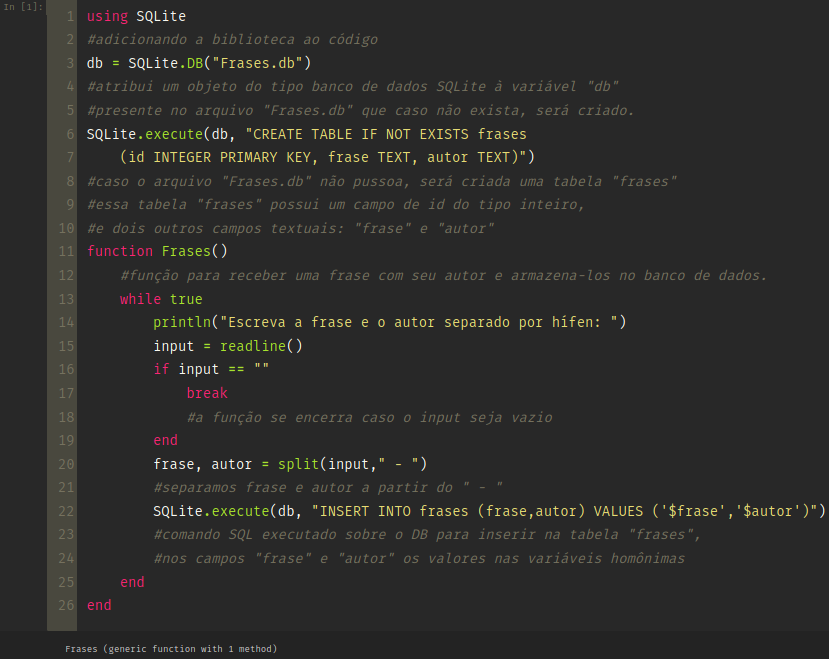
\includegraphics[width=12cm]{aplicacoes/sql_corpo.png} \\
       {\tiny \sf Fonte: Autor}
   \end{center}
\end{figure}
Em seguida executamos a função "Frases()" escrevendo três entradas de frases com seus respectivos autores conforme a figura \ref{sql_frases}. 
\begin{figure}[H]
    \begin{center}
        \caption{Função "Frases()" sendo executada} \label{sql_frases}
        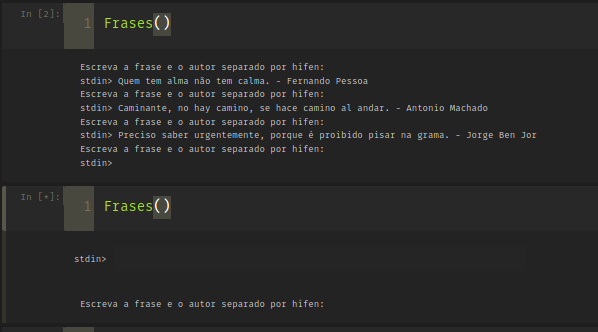
\includegraphics[width=12cm]{aplicacoes/sql_frases.png} \\
        {\tiny \sf Fonte: Autor}
    \end{center}
\end{figure}
Finalmente, na figura \ref{sql_query}, efetuamos uma busca SQL nesse banco de dados. Selecionamos todos os campos da tabela frases, e como não utilizamos o WHERE para restringir determinadas entradas, essa query retorna todo o conteúdo da tabela frases. 
Interessante notar que o comando SQLite.DBInterface.execute() retorna um objeto, que transformamos em DataFrame para o acessarmos. 

\begin{figure}[H]
   \begin{center}
       \caption{Query do banco de frases criado} \label{sql_query}
       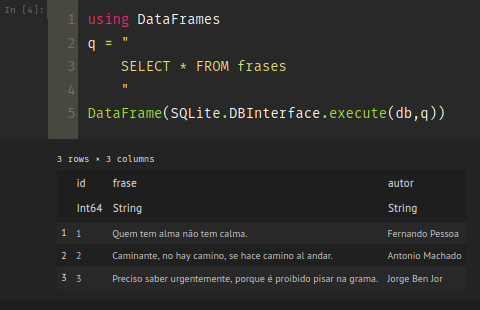
\includegraphics[width=12cm]{aplicacoes/sql_query.png} \\
       {\tiny \sf Fonte: Autor}
   \end{center}
\end{figure}
%Aqui trazemos dois exemplos de utilização do banco de dados SQLite. No primeiro nós criamos um arquivo de banco de dados, preenchemos com algumas informações e as recuperamos. Já no segundo demonstramos uma query no famoso banco de dados \href{https://github.com/lerocha/chinook-database/blob/master/ChinookDatabase/DataSources/Chinook_Sqlite.sqlite}{Chinook}, que seria em SQL o equivalente ao Iris Dataset em Data Analysis. 
%#A princípio vou deixar só o meu primeiro exemplo mesmo, pra não ter que explicar sobre o chinook e tal








%\section{Pesquisa operacional}
%Nesse exemplo utilizamos a biblioteca JuMP.jl que nos dá uma interface unificada para utilizar diversos motores de resolução de problemas lineares.






%Dataframes em julia?
%Matrizes em Julia? Linear solver? 
%Operational research? 
%Data Wrangling?
%Pesquisar nos videos do Grant 3b1b e no 



%\section{Julia Sets}
%Para esse último exemplo criamos uma aplicação que interativa que %apresenta o conjunto matemático de números complexos chamado "Julia %Set". Foi escolhido devido a sua beleza e ao nome muito propício. O %conjunto de Julia é muito próximo do ainda mais famoso conjunto de %Mandelbrot \footnote{http://paulbourke.net/fractals/juliaset/}. 
%
%Para tanto, utilizamos o ecossistema Makie.jl, um conjunto de %diversas bibliotecas e pacotes de plotagem gráfica em Julia. %Especialmente utilizada para criação de gráficos interativos ou de %altíssima qualidade para publicação em revista. 

%Nos baseamos no exemplo da biblioteca de interação com mouse. 
%Nesse capítulo apresentamos uma representação gráfica de um conjunto matemático chamado Julia Sets. Escolhemos esse exemplo pela beleza e também pelo nome, pois devido a fama desse conceito, especialmente de seu conceito irmão que é o conjunto de Mandelbrot é muito provavel que os criadores da linguagem tenham considerado o conjunto Julia como um possível reiminencia. 

%Nesse capítulo apresentamos a biblioteca Makie.jl, que é também é uma biblioteca gráfica como o Plots.jl porém mais utilizada para criação de aplicações dinâmicas ou gráficos de alta qualidade para publicação. 



%\chapterimage{Conclusao.jpg} % Chapter heading image
%\input{05conclusaoR.tex}










\chapterimage{Biblioteca.png}
\bibliographystyle{alpha}
\bibliography{Julia}
\addcontentsline{toc}{chapter}{\textcolor{purple}{Bibliografia}}



%----------------------------------------------------------------------------------------
%\newpage
%% Prof. Dr. Ausberto S. Castro Vera
% UENF - CCT - LCMAT - Curso de Ci\^{e}ncia da Computa\c{c}\~{a}o
% Campos, RJ,  2021
% Disciplina: Paradigmas de Linguagens de Programa\c{c}\~{a}o
%


\noindent
\textbf{Disciplina:} \textit{Paradigmas de Linguagens de Programa\c{c}\~{a}o 2021}\\
\textbf{Linguagem:} \textit{Linguagem R}\\
\textbf{Aluno:} \textit{Nome Completo do aluno}\\
\textbf{Data:} \today

\section*{Ficha de avalia\c{c}\~{a}o:}



\begin{tabular}{|p{12cm}|c|}
  \hline
  % after \\: \hline or \cline{col1-col2} \cline{col3-col4} ...
  \textbf{Aspectos de avalia\c{c}\~{a}o (requisitos m\'{\i}nimos)} & \textbf{Pontos} \\
  \hline
  Elementos b\'{a}sicos da linguagem (M\'{a}ximo: 01 pontos) &  \\
  $\bullet$ Sintaxe (vari\'{a}veis, constantes, comandos, opera\c{c}\~{o}es, etc.) &  \\
  $\bullet$ Usos e \'{a}reas de Aplica\c{c}\~{a}o da Linguagem &  \\
  \hline
  Cada elemento da linguagem (defini\c{c}\~{a}o) com exemplos (M\'{a}ximo: 02 pontos) &  \\
  $\bullet$ Exemplos com fonte diferenciada ( Courier , 10 pts, azul) & \\
  \hline
  M\'{\i}nimo 5 exemplos completos - Aplica\c{c}\~{o}es (M\'{a}ximo : 2 pontos) &  \\
  $\bullet$ Uso de rotinas-fun\c{c}\~{o}es-procedimentos, E/S formatadas &  \\
  $\bullet$ Menu de opera\c{c}\~{o}es, programas gr\'{a}ficos, matrizes, aplica\c{c}\~{o}es &  \\
  \hline
  Ferramentas (compiladores, interpretadores, etc.) (M\'{a}ximo : 2 pontos) &  \\
  $\bullet$ Ferramentas utilizadas nos exemplos: pelo menos DUAS&  \\
  $\bullet$ Descri\c{c}\~{a}o de Ferramentas existentes:  m\'{a}ximo 5&  \\
  $\bullet$ Mostrar as telas dos exemplos junto ao compilador-interpretador&  \\
  $\bullet$  Mostrar as telas dos resultados obtidos nas ferramentas &  \\
  $\bullet$ Descri\c{c}\~{a}o das ferramentas (autor, vers\~{a}o, homepage, tipo, etc.) &  \\
  \hline
  Organiza\c{c}\~{a}o do trabalho (M\'{a}ximo: 01 ponto) &  \\
  $\bullet$ Conte\'{u}do, Historia, Se\c{c}\~{o}es, gr\'{a}ficos, exemplos, conclus\~{o}es, bibliografia &  \\
  \hline
   Uso de Bibliografia (M\'{a}ximo: 01 ponto)&  \\
   $\bullet$ Livros: pelo menos 3&  \\
   $\bullet$ Artigos cient\'{\i}ficos: pelo menos 3 (IEEE Xplore, ACM Library)&  \\
   $\bullet$ Todas as Refer\^{e}ncias dentro do texto, tipo [ABC 04] & \\
   $\bullet$ Evite Refer\^{e}ncias da Internet & \\
   \hline
     &  \\
  Conceito do Professor (Opcional: 01 ponto) & \\
  \hline
   & \\
  \hfill Nota Final do trabalho: & \\
  \hline
\end{tabular}\\
\textit{Observa\c{c}\~{a}o:} Requisitos m\'{\i}nimos significa a \textit{metade} dos pontos


\end{document}

